\documentclass[]{article}
\usepackage{lmodern}
\usepackage{amssymb,amsmath}
\usepackage{ifxetex,ifluatex}
\usepackage{fixltx2e} % provides \textsubscript
\ifnum 0\ifxetex 1\fi\ifluatex 1\fi=0 % if pdftex
  \usepackage[T1]{fontenc}
  \usepackage[utf8]{inputenc}
\else % if luatex or xelatex
  \ifxetex
    \usepackage{mathspec}
  \else
    \usepackage{fontspec}
  \fi
  \defaultfontfeatures{Ligatures=TeX,Scale=MatchLowercase}
\fi
% use upquote if available, for straight quotes in verbatim environments
\IfFileExists{upquote.sty}{\usepackage{upquote}}{}
% use microtype if available
\IfFileExists{microtype.sty}{%
\usepackage{microtype}
\UseMicrotypeSet[protrusion]{basicmath} % disable protrusion for tt fonts
}{}
\usepackage[margin=1in]{geometry}
\usepackage{hyperref}
\hypersetup{unicode=true,
            pdfborder={0 0 0},
            breaklinks=true}
\urlstyle{same}  % don't use monospace font for urls
\usepackage{graphicx,grffile}
\makeatletter
\def\maxwidth{\ifdim\Gin@nat@width>\linewidth\linewidth\else\Gin@nat@width\fi}
\def\maxheight{\ifdim\Gin@nat@height>\textheight\textheight\else\Gin@nat@height\fi}
\makeatother
% Scale images if necessary, so that they will not overflow the page
% margins by default, and it is still possible to overwrite the defaults
% using explicit options in \includegraphics[width, height, ...]{}
\setkeys{Gin}{width=\maxwidth,height=\maxheight,keepaspectratio}
\IfFileExists{parskip.sty}{%
\usepackage{parskip}
}{% else
\setlength{\parindent}{0pt}
\setlength{\parskip}{6pt plus 2pt minus 1pt}
}
\setlength{\emergencystretch}{3em}  % prevent overfull lines
\providecommand{\tightlist}{%
  \setlength{\itemsep}{0pt}\setlength{\parskip}{0pt}}
\setcounter{secnumdepth}{5}
% Redefines (sub)paragraphs to behave more like sections
\ifx\paragraph\undefined\else
\let\oldparagraph\paragraph
\renewcommand{\paragraph}[1]{\oldparagraph{#1}\mbox{}}
\fi
\ifx\subparagraph\undefined\else
\let\oldsubparagraph\subparagraph
\renewcommand{\subparagraph}[1]{\oldsubparagraph{#1}\mbox{}}
\fi

%%% Use protect on footnotes to avoid problems with footnotes in titles
\let\rmarkdownfootnote\footnote%
\def\footnote{\protect\rmarkdownfootnote}

%%% Change title format to be more compact
\usepackage{titling}

% Create subtitle command for use in maketitle
\newcommand{\subtitle}[1]{
  \posttitle{
    \begin{center}\large#1\end{center}
    }
}

\setlength{\droptitle}{-2em}
  \title{}
  \pretitle{\vspace{\droptitle}}
  \posttitle{}
  \author{}
  \preauthor{}\postauthor{}
  \date{}
  \predate{}\postdate{}

-\usepackage[alf]{abntex2cite}

\begin{document}

{
\setcounter{tocdepth}{2}
\tableofcontents
}
\section*{Introdução}\label{introducao}
\addcontentsline{toc}{section}{Introdução}

\section{O Direito e a Economia}\label{cap:1}

Este capítulo tem como finalidade discutir os aspectos legais da
política monetária no Brasil e no mundo, partindo desde os conceitos
básicos de Estado e Constituição até a definição do regime de metas de
inflação no Brasil, em 1999, à luz do direito ao trabalho e à livre
iniciativa, passando pelos conceitos de ``Constituição Econômica'',
Economia,como ciência e como atividade, suas interações com o Direito e
a estruturação legal do Sistema Financeiro Nacional (SFN) e das suas
principais instituições, ou seja, as Autoridades Monetárias,
responsáveis pela estabilidade da moeda no Brasil, por fim comparando
suas atribuições com as atribuições do \emph{Federal Reserve} (FED).

\subsection{Conceitos de Estado e
Constituição}\label{conceitos-de-estado-e-constituicao}

Estado é uma instituição organizada politicamente, socialmente e
juridicamente, ocupando um território definido, normalmente onde a lei
máxima é uma Constituição escrita, e dirigida por um Governo que possui
soberania reconhecida tanto interna quanto externamente. O Estado é
responsável pela organização e pelo controle social, pois detém, segundo
\citeauthoronline{weber}, o monopólio legítimo do uso da força.

\begin{quote}
O Estado é uma relação de homens dominando homens, relação mantida por
meio da violência legítima (isto é, considerada como legítima). Ele é
uma comunidade humana que pretende, com êxito, o monopólio do uso
legítimo da força física dentro de um determinado território
\cite{weber}.
\end{quote}

Já \citeonline[p.~2-3, grifo nosso]{moraes}, em uma definição mais
moderna de Estado, traz:

\begin{quote}
O Estado, na tradicional obra de Jellinek, necessita de três elementos
fundamentais: poder/soberania, população e território. O Estado,
portanto, é a forma histórica de organização jurídica limitado a um
determinado território e com população definida e dotado de soberania,
que em termos gerais e \textbf{no sentido moderno configura-se em um
poder supremo no plano interno e num poder independente no plano
internacional}.
\end{quote}

De acordo com o atual Código Civil, o Estado possui personalidade
jurídica de direito público, com prerrogativas especiais, para que possa
ser atingida a finalidade de interesse público. O fim do Estado é
assegurar a vida humana em sociedade. O Estado deve garantir a ordem
interna, assegurar a soberania na ordem internacional elaborar as regras
de conduta e distribuir a justiça. Nesse contexto, insere-se o Direito
Administrativo, como ramo autônomo do Direito Público, tendo como
finalidade disciplinar as relações entre as diversas pessoas e órgãos do
Estado, bem como entre este e os administrados.

\subsubsection{Estado de Direito e Estado Democrático de
Direito}\label{estado-de-direito-e-estado-democratico-de-direito}

O conceito de \textbf{Estado de Direito} é mais restritivo que o exposto
no item anterior. Para um Estado ser considerado um Estado de Direito
deve apresentar as seguintes premissas \cite[p.~5]{moraes}:

\begin{enumerate}
\def\labelenumi{\arabic{enumi}.}
\tightlist
\item
  primazia da lei
\item
  sistema hierárquico de normas que preserva a segurança jurídica e que
  se concretiza na diferente natureza das distintas normas e em seu
  correspondente âmbito de validade
\item
  observância obrigatória da legalidade pela administração pública
\item
  separação de poderes como garantia da liberdade ou controle de
  possíveis abusos
\item
  reconhecimento da personalidade jurídica do Estado, que mantém
  relações jurídicas com os cidadãos
\item
  reconhecimento e garantias dos Direitos fundamentais incorporados à
  ordem constitucional
\item
  em alguns casos, a existência de controle de constitucionalidade das
  leis como garantia ante o despotismo do Legislativo
\end{enumerate}

Logo em seguida \citeonline[p.~6]{moraes} nos traz uma abordagem sobre o
\textbf{Estado Democrático de Direito}, que visa os direitos e as
garantias constitucionais:

\begin{quote}
Estado democrático de Direito, caracterizador do \emph{Estado
constitucional}, significa que o Estado se rege por normas democráticas,
com eleições livres, periódicas e pelo povo, bem como o respeito das
autoridades públicas aos Direitos e garantias Fundamentais é proclamado,
por exemplo, no caput do art. 1º da Constituição da República Federativa
do Brasil, que adotou, igualmente, em seu parágrafo único, o denominado
princípio democrático ao firmar que ``todo poder emana do povo, que o
exerce por meio de representantes eleitos ou diretamente, nos termos
desta constituição'', para mais adiante, em seu art. 14, proclamar que
``a soberania popular será exercida pelo sufrágio universal e pelo voto
direto e secreto, com valor igual para todos, e, nos termos da lei,
mediante: I- plebiscito; II- referendo; III- iniciativa popular.''
\end{quote}

De acordo com \apudonline[p.~6]{canotilho}{moraes}, ``assim, o princípio
democrático exprime fundamentalmente a existência da integral
participação de todos e de cada uma das pessoas na vida política do
país, a fim de garantir o respeito à soberania popular.''

``O \emph{Estado Constitucional}, portanto, é mais do que o \emph{Estado
de Direito}, é também o \emph{Estado Democrático}, introduzido no
constitucionalismo como garantia de legitimação e limitação do poder''
\cite[p.~6]{moraes}.

\subsubsection{Conceito de constituição e a
CF-88}\label{conceito-de-constituicao-e-a-cf-88}

Segundo \citeonline[p.~6]{moraes}, ``Constituição, \emph{lato sensu}, é
o ato de constituir, de estabelecer, de firmar; ou, ainda, o modo pelo
qual se constitui uma coisa, um ser vivo, um grupo de pessoas;
organização, formação.'' Para \apudonline[p.~6]{guetzevitch}{moraes},
``a Constituição de cada país é sempre um compromisso entre as tradições
políticas existentes.''

O conceito \textbf{jurídico} de constituição pode ser sintetizado nas
palavras de \apudonline[p.~6]{canotilho}{moraes}, transcritas abaixo:

\begin{quote}
Juridicamente, porém, \emph{Constituição} deve ser entendida como lei
fundamental e suprema de um Estado, que contém normas referentes à
estruturação do Estado, à formação dos Direitos públicos, forma de
governo e aquisição do poder de governar, distribuição de competências,
direitos, garantias e deveres dos cidadãos. Além disso, é a Constituição
que individualiza os órgãos competentes para a edição de normas
jurídicas, legislativas ou administrativas.
\end{quote}

A Constituição Federal de 88 pode ser classificada em:

\begin{itemize}
\tightlist
\item
  \textbf{formal e escrita}, já que foi ``consubstanciada de forma
  escrita, por meio de documento solene estabelecido pelo poder
  constituinte originário'' \cite[p.~8]{moraes}
\item
  \textbf{legal}, já que ``é o mais alto estatuto jurídico do país, ou
  seja, está no ápice da pirâmide normativa e dotada de coercibilidade''
  \cite[p.~8]{moraes}
\item
  \textbf{dogmática}, já que foi ``escrita e sistematizada por um órgão
  constituinte, à partir de princípios e ideias fundamentais da teoria
  política e do direito dominante'' \cite[p.~8-9]{moraes}
\item
  \textbf{promulgada}, já que foi fruto de uma ``Assembléia Nacional
  Constituinte eleita pelo povo com a finalidade de sua elaboração''
  \cite[p.~9]{moraes}
\item
  \textbf{rígida}, haja vista que pode ``ser alterada, mas somente
  mediante processo legislativo mais solene e dificultoso do que o
  existente para a edição das demais espécies normativas''
  \cite[p.~9]{moraes} e
\item
  \textbf{analítica}, já que ``regulamentam todos os assuntos que
  entendam relevantes à formação, destinação e funcionamento do estado''
  \cite[p.~10]{moraes}
\end{itemize}

\subsection{Do direito ao trabalho e à livre
iniciativa}\label{do-direito-ao-trabalho-e-a-livre-iniciativa}

\subsubsection{Declaração Universal de Direitos
Humanos}\label{declaracao-universal-de-direitos-humanos}

Não por acaso a Constituição Federal de 88 prevê o direito ao trabalho
como fundamento da nossa República (ver
\autoref{subsubsec:fundamentos}). Pelo menos desde o pós-guerra, o
direito ao trabalho figura nas constituições de diversos Estados
democráticos, assim como a \textbf{Declaração Universal de Direitos
Humanos (DUDH)}. Segundo a Organização das Nações Unidas (ONU), ``desde
sua adoção, em 1948, a DUDH foi traduzida em mais de 500 idiomas --- o
documento mais traduzido do mundo --- e inspirou as constituições de
muitos Estados e democracias recentes'' \cite{dudh}.

Em relação ao trabalho, a declaração da \citeonline[art.~23]{dudh}
impõe:

\begin{enumerate}
\def\labelenumi{\arabic{enumi}.}
\tightlist
\item
  Toda a pessoa tem direito ao trabalho, à livre escolha do trabalho, a
  condições eqüitativas e satisfatórias de trabalho e à proteção contra
  o desemprego.
\end{enumerate}

\subsubsection{Constituição Federal de
1988}\label{constituicao-federal-de-1988}

\begin{quote}
é através do trabalho que o homem garante sua subsistência e o
crescimento do país, prevendo a Constituição, em diversas passagens, a
liberdade, o respeito e a dignidade ao trabalhador (por exemplo: CF,
arts. 5º, XII; 6º; 7º; 8º; 194-204). Como salienta Paolo Barile, a
garantia de proteção ao trabalho não engloba somente o trabalhador
subordinado, mas também aquele autônomo e o empregador, enquanto
empreendedor do crescimento do país \apud[p.~19]{barile}{moraes}.
\end{quote}

\paragraph{Fundamentos da República Federativa do
Brasil}\label{subsubsec:fundamentos}

São fundamentos da República Federativa do Brasil, elencados no artigo
primeiro da Constituição Federal de 88 \cite[grifo nosso]{cf88}:

I - a soberania;

II - a cidadania;

III - \textbf{a dignidade da pessoa humana};

IV - \textbf{os valores sociais do trabalho e da livre iniciativa};

V - o pluralismo político.

Enfatiza-se aqui os incisos III e IV, por estarem estes intimamente
relacionados com a realidade econômica do país.

\paragraph{Objetivos fundamentais}\label{objetivos-fundamentais}

Elencam-se como objetivos fundamentais da República Federativa do
Brasil, conforme artigo 3º da CF/88 \cite[grifo nosso]{cf88}:

I - construir um sociedade livre, justa e solidária;

II - \textbf{garantir o desenvolvimento nacional};

III - \textbf{erradicar a pobreza e a marginalização e reduzir as
desigualdades sociais e regionais};

IV - promover o bem de todos, sem preconceitos de origem, raça, sexo,
cor, idade e quaisquer outras formas de discriminação.

Também aqui, como objetivos fundamentais, deve-se enfatizar a
importância de se discutir os meios segundo os quais serão promovidos
tais objetivos, em especial para este trabalho os elencados nos incisos
II e III. Não é trivial atingir objetivos como \emph{garantir o
desenvolvimento nacional}, \emph{erradicar a pobreza e a marginalização}
e ainda \emph{reduzir as desigualdades sociais e regionais}. Para isto,
faz-se necessário, a boa utilização das ciências econômicas, entre
outras.

\paragraph{Diretos Sociais}\label{diretos-sociais}

Por fim, porém não menos importante, o direito ao trabalho está
garantido através dos direitos sociais previstos na CF-88, como descrito
em seu artigo 6º:

\begin{quote}
São direitos sociais a educação, a saúde, a alimentação, o trabalho, a
moradia, o transporte, o lazer, a segurança, a previdência social, a
proteção à maternidade e à infância, a assistência aos desamparados, na
forma desta Constituição \cite[art.~6º]{cf88}.
\end{quote}

\subsubsection{A Constituição Econômica}\label{a-constituicao-economica}

Segundo \citeonline[p.~859]{moraes}, a ``Revolução Francesa e
prevalecimento das ideias liberais trouxeram o afastamento da
intervenção do Estado na economia, com a consagração das ideias de Adam
Smith.'' Porém, à partir do primeiro pós-guerra, baseadas na
Constituição de Weimar (1919), ``houve a crescente constitucionalização
do Estado Social de Direito, com a consagração em seu texto dos direitos
sociais e a previsão de aplicação e realização por parte das
instituições encarregadas desta missão'' \cite[p.~859]{moraes}.

\begin{quote}
A necessidade de regulamentação da maior intervenção estatal na
econômica (\emph{sic}), por pressão da corrente política
social-democrata nas diversas Assembléias Constituintes, gerou a
existência de previsões expressas nas diversas constituições, gerando a
denominada Constituição Econômica.Tratou-se, portanto, em um primeiro
momento da inclusão de conteúdo predominantemente programático nos
textos constitucionais, complementando o constitucionalismo nascido com
o Estado Liberal de Direito com normas relativas aos direitos sociais e
econômicos \cite[p.~859]{moraes}.
\end{quote}

Para \apudonline[p.~860]{baracho}{moraes}, atualmente, ``a relação entre
Constituição e Sistema Econômico ou mesmo Regime Econômico é frequente
nas constituições modernas'', de tal forma que podemos citar a
existência de, ``ao lado de uma constituição política, uma constituição
econômica.''

Em suma, pode-se dizer que, atualmente, há um conceito de Constituição
Econômica, como expresso por \apudonline[p.~860]{moreira}{moraes}:

\begin{quote}
A Constituição Econômica passa a designar o conjunto de preceitos e
instituições jurídicas, garantidos os elementos definidores de um
determinado sistema econômico, instituem uma determinada forma de
organização e funcionamento da economia e constituem, por isso mesmo,
uma determinada ordem econômica.
\end{quote}

No Brasil, na CF-88, a chamada ``Constituição Econômica'', ou seja, as
normas referentes à ordem econômico e financeira, pode ser encontrada no
Título VII, este subdividido em quatro capítulos, a saber: \emph{DOS
PRINCÍPIOS GERAIS DA ATIVIDADE ECONÔMICA}, \emph{DA POLÍTICA URBANA},
\emph{DA POLÍTICA AGRÍCOLA E FUNDIÁRIA} e \emph{DA REFORMA AGRÁRIA e DO
SISTEMA FINANCEIRO NACIONAL}.

No entanto, a Emenda Constitucional n.º 40 suprimiu do texto original da
CF-88 praticamente todo o capítulo que dispunha sobre o Sistema
Financeiro Nacional, que consistia tão somente do artigo 192. Com a
redação da EC n.º 40, este passou a vigorar com os seguintes dizeres
\cite{ec40}:

\textbf{Art. 192.} O sistema financeiro nacional, estruturado de forma a
promover o desenvolvimento equilibrado do País e a servir aos interesses
da coletividade, em todas as partes que o compõem, abrangendo as
cooperativas de crédito, será regulado por leis complementares que
disporão, inclusive, sobre a participação do capital estrangeiro nas
instituições que o integram \cite[art.~192]{cf88}.

Segundo \citeonline[p.~867]{moraes}, a redação deste artigo dada pela EC
nº 40/03, ``concedeu ao Congresso Nacional maior liberdade para sua
regulamentação, pois retirou a exigência de observância, por parte da
lei complementar, de diversos preceitos previstos pela redação original
do art. 192'', ou seja, a EC nº 40/03 ``desconstitucionalizou o conteúdo
básico referente ao sistema financeiro nacional'', inclusive o
estabelecido em relação no parágrafo 3º, que estabelecia uma taxa de
juros real limite de 12\% a.a..

Dentro deste Título, a valorização do trabalho humano e à livre
iniciativa são garantidos no caput do artigo 170, onde também está
estabelecido que sejam observados, entre outros, os princípios da
\cite[art. 170]{cf88}:

\begin{itemize}
\tightlist
\item
  livre-concorrência e
\item
  busca do pleno emprego
\end{itemize}

Segundo \citeonline[p.~861]{moraes}, este artigo, ``com a nova redação
que lhe deu a Emenda Constitucional nº 06/1995, consagrou a ordem
econômica, fundada na valorização do trabalho humano e na livre
iniciativa.''

\subsection{Direito e Economia}\label{sec:diretoeeconomia}

\begin{quote}
A partir de Hegel, pode-se considerar que, se o direito à liberdade
concreta for o ponto de partida da organização humana, torna-se
inexorável uma Teoria Social integrando Ética, Política, Direito e
Economia no mundo ou estado objetivo ético, denominado por Hegel
eticidade. Ele se realiza em três momentos sociais básicos: família,
sociedade civil e estado nos quais a dialética do conceito de liberdade
efetiva a eticidade \cite[p.~15]{drummond}.
\end{quote}

Nesta seção será feito um breve apanhado sobre as ciências sociais, com
foco específico nas ciências jurídicas e econômicas, além da interação
entre elas.

\subsubsection{As ciências sociais ou
humanas}\label{as-ciencias-sociais-ou-humanas}

\begin{quote}
As ciências sociais ocupam-se dos diferentes aspectos do comportamento
humano. Podem ser também caracterizadas como \textbf{ciências do
comportamento} ou, alternativamente, como \textbf{ciências humanas}.
Compreendem áreas distintas, à medida que se possam diferenciar, por sua
natureza, os diferentes aspectos da ação do homem com os quais cada uma
delas se envolve. \cite[p.~30]{rossetti}
\end{quote}

De \citeonline[p.~30-31]{rossetti}, pode-se retirar definições sucintas
das principais ciências sociais ou humanas:

\begin{enumerate}
\def\labelenumi{\arabic{enumi}.}
\tightlist
\item
  a \textbf{ciência política}, que trata das relações entre a nação e o
  Estado, das formas de governo e da condução dos negócios públicos
  \cite[p.~30]{rossetti}
\item
  a \textbf{sociologia}, que ocupa-se das relacões sociais e da
  organização estrutural da sociedade \cite[p.~30-31]{rossetti}
\item
  a \textbf{antropologia cultural}, que volta-se para o estudo das
  origens e da evolução, da organização e das diferentes formas de
  expressão cultural do homem \cite[p.~31]{rossetti}
\item
  a \textbf{psicologia}, que ocupa-se do comportamento do homem, de suas
  motivações, valores e estímulos \cite[p.~31]{rossetti}
\item
  o \textbf{direito}, ao qual cabe fixar, com precisão ditada pelos
  usos, costumes e valores da sociedade, as normas que regularão os
  direitos e as obrigações individuais e sociais \cite[p.~31]{rossetti}
\item
  a \textbf{economia}, que compete o estudo da ação econômica do homem,
  envolvendo essencialmente o processo de produção, a geração e a
  apropriação da renda, o dispêndio e a acumulação
  \cite[p.~31]{rossetti}
\item
  a \textbf{filosofia} e a \textbf{ética}, as quais cabem questionar os
  princípios e aquisições conceituais de outros campos
  \cite[p.~31]{rossetti}
\item
  a \textbf{história}, que estuda o ser humano e sua ação no tempo e no
  espaço concomitantemente à análise de processos e eventos ocorridos no
  passado \cite{historia}
\item
  e a \textbf{religião} ou \textbf{ciências da religião}, que investiga
  sistematicamente religiões em todas as suas manifestações
  \cite{religiao}
\end{enumerate}

\subsubsection{O Conceito de Economia}\label{o-conceito-de-economia}

Uma definição inicial de \textbf{economia}, haja vista ser possível
muitas definições do termo, pode ser extraída de
\citeonline[p.~5]{passosnogami}:

\begin{quote}
em termos etimológicos, a palavra ``economia'' vem do grego
\textbf{\emph{oikos}} (casa) e \textbf{\emph{nomos}} (norma, lei).
Teríamos então, a palavra \textbf{\emph{oikonomia}} que significa
``administração de uma unidade habitacional (casa)'', podendo também ser
entendida como ``administração da coisa pública'' ou se um Estado.
\end{quote}

Já em \textbf{Economia}, para \citeonline[p.~5]{passosnogami}, estuda-se
``as maneiras pelas quais os diferentes tipos de sistemas econômicos
administram seus limitados recursos com a finalidade de produzir bens e
serviços.''

\begin{quote}
A complexa teia das relações sociais e a multiplicidade dos fatores
condicionantes da atividade econômica dificultam, de certa forma, a
formulação de uma definição abrangente para a economia. Além disso, como
já destacamos, a economia é fortemente influenciada, tanto em sua
construção como ramo de conhecimento, como na realidade, por diferentes
concepções político-ideológicas, algumas até conflitantes entre si.
Conseqüentemente, cada corrente de pensamento econômico enxerga a
realidade sob ângulos diferenciados, a partir dos quais elabora suas
concepções, estabelece seus conceitos e formata seus modelos. E tem
mais: ao longo do tempo, as instituições econômicas e as concepções
político-ideológicas se modificam. Torna-se geralmente maior a
complexidade do processo econômico. Surgem novas preocupações. E evolui,
decorrentemente, o conceito de economia \cite[p.~43-46]{rossetti}.
\end{quote}

\paragraph{\texorpdfstring{Os vários significados do termo
\emph{economia}}{Os vários significados do termo economia}}\label{os-varios-significados-do-termo-economia}

\begin{quote}
A propósito da religião (que, para Marx, era a ideologia por
excelência), Hegel distinguiu três momentos: \emph{doutrina, crença e
ritual}; assim, fica-se tentado a distribuir em torno desses três eixos
a multiplicidade de ideias associadas com o termo ``ideologia'': a
ideologia como um complexo de ideias (teorias, convicções, crenças,
métodos de argumentação); a ideologia em seu aspecto externo, ou seja, a
materialidade da ideologia, os Aparelhos Ideológicos de Estado; e por
fim, o campo mais fugidio, a ideologia ``espontânea'' que atua no cerne
da própria ``realidade'' social \cite[p.~15]{zizek}.
\end{quote}

Segundo \citeonline[p.~7]{singer}, ``podemos distinguir pelo menos três
significados do termo \emph{economia}'':

\begin{itemize}
\tightlist
\item
  a qualidade de ser estrito ou austero no uso de recursos ou valores
\item
  a característica comum de uma ampla gama de atividades que compõe a
  \emph{economia} de um país, de uma cidade, etc.
\item
  a ciência que tem por objeto a atividade que dá o segundo significado
\end{itemize}

A economia (ciência) é a sistematização do conhecimento sobre a economia
(atividade).

\paragraph{A economia como atividade}\label{a-economia-como-atividade}

A ciência se divide a respeito da definição de economia como atividade,
entre social (escola \emph{marxista}) e individual (escola
\emph{marginalista}) \cite[p.~9]{singer}.

Enquanto para os \emph{marxistas} a atividade econômica é sempre
coletiva, praticada mediante a divisão social do trabalho, para os
\emph{marginalistas} a atividade econômica é em sua essência individual,
que atuam autonomamente, tendo em vista apenas seus desejos ou suas
necessidades \cite[p.~10]{singer}.

\paragraph{A economia como ciência}\label{a-economia-como-ciencia}

Também diferem os \emph{marxistas} e os \emph{marginalistas} quanto a
definição de economia como ciência.

Enquanto para os \emph{marxistas} a economia política é a ciência do
social, abrangendo em seu campo de estudo o conjunto de atividades que
formam a vida econômica da sociedade \cite[p.~14]{singer}, para os
\emph{marginalistas} a ciência econômica tem como modelo as ciências da
natureza, onde cada uma das quais tem como objeto próprio um determinado
``setor'' do universo físico. Analogamente, as ciências do homem teriam
como objeto um ``setor'' do universo humano \cite[p.~15]{singer}.

Para \citeauthoronline{rangel1956}, ``ciência é classificação e medida
-- não apenas medida, como pode se depreender do lema econométrico. Se
ciência fosse medida não haveria ciência em Aristóteles ou Hegel''
\cite[p.~204]{rangel1956}.

A evolução da economia, segundo \citeonline{rangel1956}, dá-se através
de um duplo processo evolutivo, o fenomenal e o numenal, seguindo a
filosofia de Kant:

\begin{quote}
a economia é uma ciência histórica por excelência -- qualidade que
partilha com outras ciências sociais. Quer isso dizer que está submetida
a um duplo processo evolutivo: o fenomenal (como representação, como
ideia da coisa, como ``coisa para nós'', no sentido kantiano) e o
numenal (como objeto, coisa representada, ``coisa em si'')
{[}\ldots{}{]} e não pode ser estudada senão nesse duplo contexto
\cite[p.~204]{rangel1956}.
\end{quote}

\subsubsection{A Economia como Ciência
Social}\label{a-economia-como-ciencia-social}

Como Ciência Social, a Economia pode ser definida como a ciência:

\begin{quote}
que estuda como as pessoas e a sociedade decidem empregar recursos
escassos, que poderiam ter utilização alternativa, na produção de bens e
serviços de modo a distribuí-los entre as várias pessoas e grupos da
sociedade, a fim de satisfazer as necessidades humanas
\cite[p.~5]{passosnogami}.
\end{quote}

Para \citeonline[p.~31]{rossetti}, no entanto, a Economia não é uma
ciência com limites nitidamente definidos, assim como as demais ciências
sociais:

\begin{quote}
À semelhança do que ocorre com os demais ramos das ciências sociais, não
se pode considerar a economia como fechada em torno de si mesma. Pelas
implicações da ação econômica sobre outros aspectos da vida humana, o
estudo da economia implica a abertura de suas fronteiras às demais áreas
das ciências humanas. Esta abertura se dá em dupla direção, assumindo
assim caráter \textbf{biunívoco}.
\end{quote}

Segundo \citeonline[p.32]{rossetti}, a separação das ciências sociais em
especialidades distintas é não-rigorosa, ou, ao contrário, estas
especialidades estão entremeadas:

\begin{quote}
Em síntese, pode-se inferir que as interfaces da economia com outros
ramos do conhecimento social decorrem de que as relações humanas e os
problemas nelas implícitos ou delas decorrentes não são facilmente
separáveis segundo níveis de referência rigorosamente pré-classificados.
O referencial econômico deve ser visto apenas como uma abstração útil,
para que se analisem aspectos específicos da luta humana pela
sobrevivência, prosperidade, bem-estar individual e bem-comum. Ocorre,
todavia, que essa mesma luta não se esgota nos limites do que se
convencionou chamar de relações econômicas. Vai muito além, abrangendo
aspectos que dizem respeito à postura ético-religiosa, às formas de
organização política, aos modos de relacionamento social, à estruturação
da ordem jurídica, aos padrões das conquistas tecnológicas, às
limitações impostas pelas condições do meio ambiente e, mais
abrangentemente, à formação cultural da sociedade.
\end{quote}

\subsubsection{A Economia e o Direito}\label{a-economia-e-o-direito}

\citeonline[p.~467]{rangel1985b} discorre a respeito da ineficácia do
uso da força da lei para fixação de variáveis econômicas, como a taxa de
juros:

\begin{quote}
As leis que busquem fazer isso são virtualmente inúteis {[}\ldots{}{]}
porque sabemos que a eficácia das leis é muito relativa e, na maior
parte dos casos, elas não passam mesmo de atos homologatórios de
mudanças, no fundamental, já acontecidas. Quando não são natimortas,
como acontece com aquelas que pretendem disciplinar matérias para o que
não se criaram ainda -- ou não existem mais -- condições objetivas.
\end{quote}

Mas observa que não o são (inúteis) ``aquelas que busquem
competentemente influir sobre as condições objetivas a que me referi.
Por exemplo, as leis que disciplinem a qualidade da garantia dos papéis
de crédito em circulação no mercado.''

\begin{quote}
Mas isto é assunto para ciência. Ciência econômica e ciência jurídica,
nada tendo em comum com esse pseudojuridicismo que imagina que tudo se
pode fazer por decreto \cite[p.~467]{rangel1985b}.
\end{quote}

E desenvolve um exemplo do uso eficiente da lei para um eficiente manejo
das variáveis econômicas:

\begin{quote}
nossos serviços de utilidade pública estão organizados como serviços
públicos concedidos a empresas públicas. Por exigência legal
{[}\ldots{}{]} esses serviços não podem usar, para a garantia de seus
papéis de crédito, a hipoteca dos bens comprometidos na prestação dos
ditos serviços de utilidade pública \cite[p.~469]{rangel1985b}.
\end{quote}

Para contornar este problema, segundo \citeonline[p.~469]{rangel1985b},
``o Estado passou, sistematicamente a conceder o seu aval --- uma
garantia fidejussória e não real, portanto ---, para a cobertura das
operações de crédito das empresas públicas{[}\ldots{}{]}'', com lastro
em ``recursos fiscais e parafiscais futuros.''

Estes recursos fiscais e parafiscais futuros, segundo
\citeonline[p.~469]{rangel1985b}, ``{[}\ldots{}{]}somente serão
cobráveis a prazos cada vez mais longos, com inevitáveis reflexos sobre
a taxa de juros, a qual, ao elevar-se {[}\ldots{}{]} esvazia a garantia
fidejussória oferecida'', o que, segundo ele, àquela época, tornaria o
custo dos serviços públicos proibitivos.

\citeauthoronline{rangel1985b} ainda prevê que:

\begin{quote}
Breve teremos uma Constituinte e, se esta não tiver que ser um desses
bate-papos inconseqüentes que nos acontecem frequentemente, deverá
cuidar desse problema e conduzir à única solução possível, que será a
privatização dos serviços de utilidade pública, única maneira de cortar
o nó górdio de nossa presente problemática econômica e, também,
jurídica, política e social, no sentido mais lato. Tudo isso envolve
complicadas questões jurídicas, mas nada que se pareça com o primarismo
de supor que se podem fixar as taxas de juros por decreto
\cite[p.~469]{rangel1985b}.
\end{quote}

Em outro artigo \cite[p.~717]{rangel1987}, \citeauthoronline{rangel1987}
afirma que ``{[}\ldots{}{]} embora sem plano concebido, o enquadramento
institucional{[}\ldots{}{]}'' (dos serviços de utilidade pública) foram
mudando, numa ``{[}\ldots{}{]} ordem perfeitamente lógica, a saber:
(a)serviços públicos concedidos a empresas privadas estrangeiras; (b)
serviços públicos de administração direta do Estado; (c) serviços
públicos concedidos a empresas públicas.''

No entanto, o ``uso do crédito garantido pelos recursos fiscais futuros,
levado além do razoável, colocou-o {[}\ldots{}{]}'' (o Estado)
``{[}\ldots{}{]} na condição de devedor insolvente''
\cite[p.~718]{rangel1987}.

\citeonline[p.~718]{rangel1987} afirma ainda que ``o novo enquadramento
institucional, que deverá tomar o lugar do caduco instituto da concessão
do serviço público a empresa pública {[}\ldots{}{]}'', seria ``a
conversão da concessão do serviço público a empresa pública, em
concessão do mesmo serviço público a empresa privada {[}\ldots{}{]}.''

\begin{quote}
Com efeito, o concessionário privado poderá emitir títulos com garantia
hipotecária. Essa garantia será oferecida ao Estado, o único tomador
possível dos ativos comprometidos na prestação de serviços públicos, em
troca de seu aval. Não mais o atual e desmoralizado aval, coberto pela
promessa de recursos fiscais futuros, mas um aval hipotecariamente
garantido, porque o Estado passará a assumir a dupla função de poder
concedente e credor hipotecário, em vez de sua presente posição de
devedor insolvente \cite[p.~719]{rangel1987}.
\end{quote}

Segundo \citeonline[p.~718]{rangel1987}, estes serviços públicos são:
``{[}\ldots{}{]} atividades monopólicas, isto é, cujos preços não podem
ser estabelecidos pela concorrência, de resto inexistente. Os preços de
tais serviços são estabelecidos através de tarifas, fixadas pelo poder
concedente'', que ``{[}\ldots{}{]} poderá ser maior ou menor do que o
custo, sendo a diferença, no primeiro caso, uma forma de imposto, embora
cobrado, não pelos guichês do Tesouro, mas pelos do concessionário e, no
segundo caso, um subsídio a ser pago pelo Tesouro {[}\ldots{}{]}''
\cite[p.~721]{rangel1987}.

Para que isto ocorra, segundo \citeonline[p.~721]{rangel1987}, ``a
legislação a vigorar deverá conduzir à fixação correta e transparente
desses parâmetros estratégicos: (a) custo do serviço; (b) tarifa a
viger.''

\subsection{Legislação e competências}\label{legislacao-e-competencias}

Esta seção trata da legislação brasileira que rege a economia nacional,
bem como do funcionamento das principais instituições responsáveis pelo
bom funcionamento da mesma. Na \autoref{subsec:SFN} será analisada a
conceituação de Sistema Financeiro Nacional, sua evolução histórica,
desde a chegada da Família Real até os dias atuais, bem como sua atual
estrutura legal. Na \autoref{subsec:aut_mon} são mostradas as principais
atribuições legais das autoridades monetárias brasileiras. Na
\autoref{subsec:pol_mon_br}, são discutidos as leis e os princípios
econômicos que regem a política monetária no Brasil, enquanto na
\autoref{subsec:pol_mon_mun} é mostrado o que ocorre em outros países do
globo em relação à matéria.

\subsubsection{Sistema Financeiro Nacional}\label{subsec:SFN}

\paragraph{Conceituação}\label{conceituacao}

Segundo \citeonline[p.~16]{fortuna2015}, ``uma conceituação bastante
abrangente de sistema financeiro poderia ser a de um conjunto de
instituições que se dedicam, de alguma forma, ao trabalho de propriciar
condições satisfatórias para a manutenção de um fluxo de recursos entre
poupadores e investidores''.

O \textbf{mercado financeiro}, ``onde se processam essas transações
{[}\ldots{}{]} pode ser considerado com o elemento dinâmico no processo
de crescimento econômico, uma vez que permite a elevação das taxas de
poupança e investimento'' \cite[p.~16]{fortuna2015}.

O sistema financeiro nacional está subdividido em diversos grupos de
instituições, a saber \cite[p.~18]{fortuna2015}:

\begin{itemize}
\tightlist
\item
  \textbf{Autoridades Monetárias}: do qual fazem parte o Conselho
  Monetário Nacional (CMN) e o Banco Central do Brasil (BC ou Bacen)
\item
  \textbf{Autoridades de apoio}: do qual fazem parte a Comissão de
  Valores Mobiliários (CVM), o Banco do Brasil (BB), o Banco Nacional de
  Desenvolvimento Econômico e Social (BNDES), a Caixa Econômica Federal
  (CEF ou Caixa) e o Conselho de Recursos do Sistema Financeiro Nacional
  (CRSFN)
\item
  \textbf{Instituições Financeiras}: sejam elas monetárias (bancos
  comerciais, Caixas Econômicas, Bancos Cooperativos e Cooperativas de
  Crédito), não monetárias (bancos de desenvolvimento, bancos de
  investimento, sociedades de crédito, etc.) ou instituições auxiliares
  do Mercado Fianceiro (Sociedades Corretoras de Títulos e Valores
  Mobiliários, Sociedades Distribuidoras de Títulos e Valores
  Mobiliários, Sociedades de Arrendamento Mercantil, Agências de Fomento
  ou Desenvolvimento e Investidores Institucionais)
\item
  \textbf{Sistema Financeiro da Habitação (SFH)}: atualmente operado
  pela Caixa, após a extinção do BNH (Decreto-Lei 2.291, de 21/11/1986)
\item
  \textbf{Superintendência Nacional de Previdência Complementar
  (PREVIC)}
\item
  \textbf{Superintendência de Seguros Privados (SUSEP)}
\end{itemize}

\paragraph{Origem e Evolução
Histórica}\label{origem-e-evolucao-historica}

Segundo \apudonline[p.~12]{brito2005}{beatrizselan}, as quatro grandes
fases que marcaram a evolução histórica do sistema financeiro nacional
foram:

A. Da Família Real até a Primeira Guerra Mundial (1808 -- 1914). B. Da
Primeira Guerra Mundial até a Segunda Guerra Mundial (1914 -- 1945). C.
Após a Segunda Guerra Mundial até a Grande Reforma Financeira (1945 --
1964). D. Da Grande Reforma Financeira até hoje (1.964 -- nossos dias)

A primeira fase marcou-se pela abertura dos portos, com acordos
comerciais diretamente entre as partes envolvidas; a segunda fase em
conjunto com a permissão para instalação de bancos estrangeiros no
país.\cite[p.~12]{beatrizselan}

Na segunda fase criou-se a Inspetoria Geral de Bancos, em 1.920 e a
Câmara de Compensação, em 1.921, que resultou no fortalecimento dos
critérios e normas para atividade de intermediação financeira, com
consequente crescimento da atividade bancária no país
\cite[p.~12]{beatrizselan}.

Na terceira fase, com a criação da Superintendência da Moeda e do
Crédito (Sumoc), com função de supervisão e controle do mercado
monetário e a criação do Banco Nacional de Desenvolvimento Econômico e
Social (BNDES), com o objetivo de fornecer créditos de longo prazo e a
substituição de importações \cite[p.~12]{beatrizselan}.

\paragraph{Estrutura legal}\label{estrutura-legal}

No Brasil, até 1964, ``o Sistema Financeiro Nacional -- SFN -- carecia
de uma estruturação racional adequada às necessidades e carências da
sociedade como um todo. A partir de então, foi editada uma série de leis
que possibilitou esse reordenamento'' \cite[p.~15-16]{fortuna2015}:

\begin{itemize}
\tightlist
\item
  Lei da Correção Monetária (4.357/64) \cite{brasil1964a}
\item
  Lei do Plano Nacional da Habitação (4.380/64) \cite{brasil1964b}
\item
  Lei da Reforma do Sistema Financeiro Nacional (4.595/64)
  \cite{brasil1964c}
\item
  Lei do Mercado de Capitais (4.728/65) \cite{brasil1965}
\item
  Lei da CVM (6.385/76) \cite{brasil1976a}
\item
  Lei das S.A. (6.404/76) \cite{brasil1976b}
\item
  Nova Lei das S.A. (10.303/01) \cite{brasil2001a}
\item
  Decreto 3.995/01 \cite{brasil2001b}\footnote{No original, uma
    incorreção: \citeauthoronline{fortuna2015} cita o \emph{decreto
    3.995 de 31/10/2002}, quando na verdade o decreto é de 31/10/2001.}
\item
  Lei 10.411/02 \cite{brasil2002}\footnote{O original cita a MP8/2002
    (na verdade seria MP8/2001). Esta, após análise do congresso
    nacional, se transformou na lei citada.}
\item
  Resolução CMN 3.040/02 \cite{bcb2002}
\end{itemize}

\paragraph{A Lei da Correção
Monetária}\label{a-lei-da-correcao-monetaria}

Segundo \citeonline[p.~15]{fortuna2015}, a lei de correção monetária
``instituiu normas para a indexação de débitos fiscais, criou títulos
públicos federais com cláusula de correção monetária (ORTN) --
destinados a antecipar receitas, cobrir déficit público e promover
investimentos''.

\begin{quote}
Historicamente, a inflação brasileira superava os 12\% ao ano e, com
base no Direito Canônico, a Lei da Usura limitava os juros a 12\% ao
ano. As empresas e os indivíduos preferiam aplicar seus recursos
disponíveis em outras alternativas, adiando, inclusive, o pagamento de
suas obrigações tributárias. A mesma limitava a capacidade do Poder
Público de financiar-se mediante a emissão de títulos próprios, impondo
a emissão primária de moeda para satisfazer as necessidades financeiras
\cite[p.~15]{fortuna2015}.
\end{quote}

Segundo \citeauthoronline{rangel1983}, a correção monetária não foi
criada com a lei 4.357/64, que apenas legalizou o que há muito já se
praticava:

\begin{quote}
A correção monetária, que me lembre, não nasceu em 1964, quando a dupla
Campos-Bulhões a fez promulgar, pelo punho de Castelo, mas seis ou sete
anos antes, quando o mesmo grupo instituiu, pelo punho de Juscelino, o
princípio da inclusão da diferença cambial na tarifa dos serviços de
utilidade pública de eletricidade. Isto sem falarmos naquela ``correção
monetária'' hostil a qualquer cálculo econômico sério , que sempre se
praticou, sob a forma da inclusão do montante dos mútuos de um
diferencial de preços somente explicável como antecipação da inflação
futura. Esse diferencial que é o verdadeiro vilão na presente crise do
sistema nacional de habitação \cite[p.~411]{rangel1983}.
\end{quote}

\citeonline[p.~411]{rangel1983} ainda argumenta que a correção monetária
teve o mérito de criar:

\begin{quote}
a possibilidade de um cálculo econômico razoavelmente sério, sob cuja
égide criamos, em brevíssimo prazo, um dos maiores sistemas de poupança
do mundo, sem o qual seria muito difícil explicar o chamado ``milagre do
Delfim'', que elevou a taxa de crescimento do PIB a mais de 10\%,
trazendo, ao mesmo tempo, a taxa de inflação, de mais de 100, a menos de
20\% ao ano.
\end{quote}

\paragraph{A Lei do Plano Nacional de
Habitação}\label{a-lei-do-plano-nacional-de-habitacao}

Como tentativa de solucionar o déficit habitacional urbano no Brasil,
foi criado o Banco Nacional da Habitação (BNH).

\begin{quote}
A articulação deste sistema resultou da necessidade de gerar condições
para a intermediação de recursos financeiros no específico setor da
construção de habitações e urbanização/saneamento, tendo em vista o
violento crescimento populacional urbano \cite[p.~44]{fortuna2015}.
\end{quote}

Em 1986, através do decreto-lei 2.291 \cite{brasil1986}, foi decretada a
extinção do BNH e sua incorporação à Caixa Econômica Federal, mantendo
as mesmas atribuições do BNH.

\begin{quote}
foi criado o Banco Nacional de Habitação (BNH), órgão gestor do também
criado Sistema Brasileiro de Poupança e Empréstimo (SBPE), destinado a
fomentar a construção de casas populares e obras de saneamento e
infraestrutura urbana, com moeda própria {[}\ldots{}{]} e seus próprios
instrumentos de captação de recursos -- Letras Hipotecárias, Letras
Imobiliárias e Cadernetas de Poupança. Posteriormente, a esses recursos
foram adicionados os do Fundo de Garantia por Tempo de Serviço -- FGTS
\cite[p.~15]{fortuna2015}.
\end{quote}

\paragraph{Lei da Reforma do Sistema Financeiro
Nacional}\label{lei-da-reforma-do-sistema-financeiro-nacional}

Através desta lei foi criado o Conselho Monetário Nacional (CMN) e o
Banco Central do Brasil (BCB ou Bacen), segundo
\citeonline[p.~15]{fortuna2015}, com o objetivo de descentralizar a
``gestão da política monetária, de crédito e finanças públicas'', então
concentrados sob o ``Ministério da Fazenda, na Superintendência da Moeda
e do Crédito -- SUMOC -- e no Banco do Brasil.'' Para
\citeauthoronline{fortuna2015}, ``essa estrutura não correspondia aos
crescentes encargos e responsabilidades na condução da política
econômica.''

\paragraph{Lei do Mercado de Capitais}\label{lei-do-mercado-de-capitais}

Segundo \citeonline[p.~15]{fortuna2015}, com a edição desta lei foram
``estabelecidos normas e regulamentos básicos para a estruturação de um
sistema de investimentos destinado a apoiar o desenvolvimento nacional e
atender à crescente demanda por crédito''.

\paragraph{Lei da CVM}\label{lei-da-cvm}

Através desta lei foi ``criada a Comissão de Valores Mobiliários -- CVM
--, transferindo do Banco Central a responsabilidade pela regulamentação
e fiscalização das atividades relacionadas ao mercado de valores
mobiliários (ações, debêntures, etc.)'' \cite[p.16]{fortuna2015}.

\paragraph{Lei das S.A.}\label{lei-das-s.a.}

A lei das S.A. foi criada para ``atualizar a legislação sobre as
sociedades anônimas brasileiras'', estabelecendo ``regras claras quanto
às características, forma de constituição, composição acionária,
estrutura de demonstrações financeiras, obrigações societárias, direitos
e obrigações de acionistas e órgãos estatutários e legais''
\cite[p.~16]{fortuna2015}.

\paragraph{Nova lei das S.A., decreto 3.995/01 e Lei
10.411/02}\label{nova-lei-das-s.a.-decreto-3.99501-e-lei-10.41102}

Consolidação dos dispositivos da Lei da CVM e da Lei das S.A.,
melhorando a proteção aos minoritários e dando força à atuação da CVM
como órgão regulador e fiscalizador do mercado de capitais, incluindo os
fundos de investimento e os mercados de derivativos
\cite[p.~14]{beatrizselan}.

\subsubsection{Autoridades Monetárias}\label{subsec:aut_mon}

\paragraph{Conselho Monetário Nacional
(CMN)}\label{conselho-monetario-nacional-cmn}

Para \citeonline[p.~19]{fortuna2015}, o CMN, ``como órgão normativo, por
excelência, não lhe cabem funções executivas, sendo o responsável pela
fixação das diretrizes das políticas monetária, creditícia e cambial do
País. Pelo envolvimento destas políticas no cenário econômico nacional,
o CMN acaba se transformando num conselho de política econômica.''

De acordo com a lei n.º 4.595 de 31 de dezembro de 1964
\cite[art. 3º]{brasil1964c}, quanto ao Conselho Monetário Nacional
(CMN), dispõe a legislação em vigor, que sua política objetivará:

I - Adaptar o volume dos meios de pagamento às reais necessidades da
economia nacional e seu processo de desenvolvimento;

II - Regular o valor interno da moeda, para tanto prevenindo ou
corrigindo os surtos inflacionários ou deflacionários de origem interna
ou externa, as depressões econômicas e outros desequilíbrios oriundos de
fenômenos conjunturais;

III - Regular o valor externo da moeda e o equilíbrio no balanço de
pagamento do País, tendo em vista a melhor utilização dos recursos em
moeda estrangeira;

IV - Orientar a aplicação dos recursos das instituições financeiras,
quer públicas, quer privadas; tendo em vista propiciar, nas diferentes
regiões do País, condições favoráveis ao desenvolvimento harmônico da
economia nacional;

V - Propiciar o aperfeiçoamento das instituições e dos instrumentos
financeiros, com vistas à maior eficiência do sistema de pagamentos e de
mobilização de recursos;

VI - Zelar pela liquidez e solvência das instituições financeiras;

VII - Coordenar as políticas monetária, creditícia, orçamentária, fiscal
e da dívida pública, interna e externa.

A lei 12.543/2011 \cite[art. 1º]{brasil2011} ainda trata de designar ao
CMN a função de estabelecer, para fins da política monetária e cambial,
condições específicas para negociação de contratos derivativos,
independentemente da natureza do investidor, podendo, inclusive:

\begin{enumerate}
\def\labelenumi{\alph{enumi}.}
\tightlist
\item
  determinar depósitos sobre os valores nocionais dos contratos; e
\item
  fixar limites, prazos e outras condições sobre as negociações dos
  contratos derivativos.
\end{enumerate}

E, finalmente, com o decreto n.º 3088 de 21 de junho de 1999
\cite{brasil1999}, coube mais uma vez ao CMN a função de estabelecer as
\textbf{metas de inflação} e os respectivos intervalos de tolerância.

Ao longo do tempo o CMN teve a sua composição alterada, ``de acordo com
as exigências políticas e econômicas de cada momento''
\cite[p.~19]{fortuna2015}.

Com o Plano Real, por exemplo, através da Medida Provisória 542
\cite{brasil1994}, posteriormente convalidada pela lei 9.069
\cite{brasil1995}, foi simplificada a composição do CMN,
``caracterizando seu perfil monetário, que passou a ser integrado pelos
seguintes membros: Ministro da Fazenda (Presidente), Ministro do
Planejamento, Orçamento e Gestão, e Presidente do Banco Central''
\cite[p.~19]{fortuna2015}.

\paragraph{Banco Central do Brasil -- BC ou
Bacen}\label{banco-central-do-brasil-bc-ou-bacen}

Segundo \citeonline[p.~20]{fortuna2015}, O BC foi criado ``para atuar
como órgão executivo central do sistema financeiro''.

No Brasil compete ao Banco Central da República do Brasil (Bacen),
segundo a lei n.º4.595 de 31 de dezembro de 1964 \cite{brasil1964c}:
``cumprir e fazer cumprir as disposições que lhe são atribuídas pela
legislação em vigor e as normas expedidas pelo Conselho Monetário
Nacional''.

São de sua privativa competência \cite[p.21]{fortuna2015}:

\begin{itemize}
\tightlist
\item
  emitir papel-moeda e moeda metálica nas condições e limites
  autorizados pelo CMN;
\item
  executar os serviços do meio circulante
\item
  receber os recolhimentos compulsórios dos bancos comerciais e os
  depósitos voluntários das instituições financeiras e bancárias que
  operam no País
\item
  realizar operações de redesconto e empréstimo às instituições
  financeiras dentro de um enfoque de política econômica do Governo ou
  como socorro a problemas de liquidez
\item
  regular a execução dos serviços de compensação de cheques e outros
  papéis;
\item
  efetuar, como instrumento de política monetária, operações de compra e
  venda de títulos públicos federais
\item
  emitir títulos de responsabilidade própria, de acordo com as condições
  estabelecidas pelo CMN
\item
  exercer o controle de crédito sob todas as suas formas;
\item
  exercer a fiscalização das instituições financeiras, punindo-as quando
  necessário;
\item
  autorizar o funcionamento, estabelecendo a dinâmica operacional, de
  todas as instituições financeiras
\item
  estabelecer as condições para o exercício de quaisquer cargos de
  direção nas instituições financeiras privadas
\item
  vigiar a interferência de outras empresas nos mercados financeiros e
  de capitais;
\item
  controlar o fluxo de capitais estrangeiros, garantindo o correto
  funcionamento do mercado cambial, operando, inclusive, via outro,
  moeda ou operações de crédito no exterior
\item
  determinar periodicamente, via Comitê de Política Monetária -- Copom,
  a taxa de juros de referência para as operações de um dia com títulos
  públicos -- a taxa SELIC e
\item
  formalizar e institucionalizar de forma complementar ao Copom, via
  Comitê de Estabilidade Financeira -- Comef, os processos formais de
  discussão interna, divulgando o Relatório de Estabilidade Financeira
  com o foco de apresentar a sua visão do sistema financeiro e das suas
  condições de risco, reforçando o conceito de que o BC tem duas
  instâncias decisórias para cumprir seus dois principais objetivos:
  garantir a estabilidade do sistema financeiro e resguardar o poder de
  compra da moeda
\end{itemize}

\subsubsection{A Política Monetária no Brasil}\label{subsec:pol_mon_br}

\paragraph{Metas de inflação}\label{metas-de-inflacao}

De acordo com \citeonline[p.~509]{blanchard}, ``em muitos países, bancos
centrais definiram como objetivo principal atingir uma taxa de inflação
baixa, tanto no curto prazo quanto no médio prazo. Isso é conhecido como
\emph{metas de inflação}.''

Segundo \citeonline[p.~60]{fortuna2015}, ``a partir do segundo semestre
de 1999, a política monetária no Brasil passou a ser subordinada ao
conceito de \emph{Inflation Targeting} ou Meta de Inflação'' e as ``suas
sistemáticas são estabelecidas por decreto presidencial e servem como
diretriz para a política monetária, além de calibrar a liquidez da
economia de forma a assegurar o crescimento econômico sustentado''.

\begin{quote}
Assim, por lei, o BC tem a obrigação de usar todos os meios necessários
de política monetária para a obtenção destas metas, sendo o principal
deles a definição periódica da taxa Selic que serve de referência para
as demais taxas de juros da economia. Uma vez estabelecidas, elas não
podem ser alteradas, seja por choques externos ou internos
\cite[p.~60]{fortuna2015}.
\end{quote}

As metas são definidas pelo CMN por proposta do Ministro da Fazenda, tem
um intervalo de tolerância para cima e para baixo e o índice escolhido
para a referência de inflação é o IPCA do IBGE, em qualquer tipo de
expurgo \cite[p.~60]{fortuna2015}.

De acordo com \citeonline[p.~60]{fortuna2015}, ``o estabelecimento do
sistema de metas provocou mudanças no funcionamento do Copom e obrigou o
BC a produzir e divulgar a cada trimestre civil um `Relatório de
Inflação'\,''.

\begin{quote}
Este documento, que é de conhecimento público, aborda o desempenho do
sistema de metas, os resultados das decisões anteriores de política
monetária e uma avaliação futura da inflação, ou seja, qual a tendência
dos índices e, se for o caso, a necessidade de correção de sua
trajetória para a adequação da meta. Graças a este relatório, o sistema
de metas fica transparente para o público e gera a confiança e a
participação necessárias ao sucesso, de forma que toda a sociedade dê a
sua contribuição possível para a convergência à meta de inflação
\cite[p.60-61]{fortuna2015}.
\end{quote}

\paragraph{Copom}\label{copom}

Segundo \citeonline[p.~61]{fortuna2015}, o Copom é composto pelos oito
membros da Diretoria Colegiada do BC, com direito a voto, sendo
presidido pelo presidente do BC, que tem o voto de qualidade.

\begin{quote}
A criação do Copom buscou proporcionar maior transparência e ritual
adequado ao processo decisório da autoridade monetária, a exemplo do que
já era adotado pelo \emph{Federal Open Market Committee} (FOMC), do
\emph{Federal Reserve}, nos Estados Unidos, e pelo \emph{Central Bank
Council}, do \emph{Bundesbank}, na Alemanha, procedimento também
adotado, em 06/1998, pelo \emph{Bank of England} na Inglaterra, com a
criação do seu \emph{Monetary Policy Committee} (MPC), assim como pelo
Banco Central Europeu desde a criação da moeda única, em 01/99
\cite[p.~61]{fortuna2015}.
\end{quote}

\subsubsection{A Política Monetária no mundo}\label{subsec:pol_mon_mun}

Segundo \citeonline{inflationtargeting} há no mundo 27 países que adotam
o sistema de metas de inflação integralmente, sendo que os pioneiros
foram a Nova Zelândia, o Canadá e o Reino Unido. ``The first three
countries to implement fully-fledged inflation targeting were New
Zealand, Canada and the United Kingdom in the early 1990s, although
Germany had adopted many elements of inflation targeting
earlier''\footnote{Os primeiros três países a implementar a meta de
  inflação integral foram a Nova Zelândia, o Canadá e o Reino Unido no
  início dos anos 90, embora a Alemanha tivesse adotado muitos elementos
  do (sistema de) metas de inflação antes.}.

Entre os mais importantes bancos centrais do mundo, é importante citar o
\emph{Federal Reserve} e o Banco Central Europeu, embora estes não sei
considerem como tal, apesar de declararem publicamente buscar uma meta
\cite{inflationtargeting}.

\paragraph{Estados Unidos da América --
EUA}\label{estados-unidos-da-america-eua}

Nos EUA, os autores do \emph{Federal Reserve Act} propositadamente
rejeitaram o conceito de um único banco central.

Em vez disso, eles previram um sistema com três características
principais \cite{fed1}:

\begin{enumerate}
\def\labelenumi{\arabic{enumi}.}
\tightlist
\item
  um Conselho de administração central
\item
  uma estrutura operacional descentralizada de 12 \emph{Reserve Banks},
  e
\item
  uma combinação de características públicas e privadas
\end{enumerate}

Embora partes do \emph{Federal Reserve System} compartilhem algumas
características com entidades do setor privado, o Federal Reserve foi
criado para servir Interesse público.

Existem três entidades-chave no \emph{Federal Reserve System}: o
\emph{Board of Governors}, os \emph{Reserve Banks} e o \emph{Federal
Open Market Committee} (FOMC). O \emph{Board of Governors}, um órgão do
governo federal que reporta e está diretamente responsável perante o
Congresso , fornece orientação geral para o Sistema e supervisiona os 12
\emph{Reserve Banks}.

\paragraph{O Federal Open Market Committee --
FOMC}\label{o-federal-open-market-committee-fomc}

O \emph{Federal Open Market Committee} (FOMC), órgão no qual muito
provavelmente o Brasil se baseou para estruturar o nosso órgão
equivalente -- o Copom --, consiste de doze membros -- sete membros do
\emph{Board of Governors} do \emph{Federal Reserve System}; o presidente
do \emph{Federal Reserve Bank of New York}; e quatro dos onze
presidentes dos outros \emph{Reserve Banks} remanescentes --, que se
revezam no período de um ano. Presidentes não-votantes assistem às
reuniões do Comité, participam nas discussões e contribuem para a
avaliação do Comité sobre a economia e as opções políticas.

O \emph{Federal Reserve} controla as três ferramentas da política
monetária -- operações de mercado aberto, a taxa de juros básica, e os
depósitos compulsórios. Enquanto o \emph{Board of Governors} do
\emph{Federal Reserve System} é responsável pela taxa de desconto e
depósitos compulsórios, o FOMC é responsável pelas operações de mercado
aberto. \footnote{Ver
  \href{https://www.federalreserve.gov/monetarypolicy/fomc.htm}{www.federalreserve.gov/monetarypolicy/fomc.htm}.}

\paragraph{O Federal Reserve Board of
Governors}\label{o-federal-reserve-board-of-governors}

O \emph{Board of Governors} -- ou Conselho de ``Governantes'' do FED --,
localizado em Whashington, D.C., é o corpo do \emph{Federal Reserve
System}. É dirigido por sete membros, ou ``governantes'', que são
nomeados pelo presidente dos EUA e confirmados pelo Senado americano. O
Conselho orienta o funcionamento do \emph{Federal Reserve System} para
promover os objetivos e cumprir as responsabilidades atribuídas ao
\emph{Federal Reserve} pelo \emph{Federal Reserve Act} \cite{fed2}.

\begin{quote}
The FOMC is charged with overseeing ``open market operations'', the
principal tool by which the Federal Reserve executes U.S. monetary
policy. These operations affect the federal funds rate, which in turn
influence overall monetary and credit conditions, aggregate demand, and
the entire economy. The FOMC also directs operations undertaken by the
Federal Reserve in foreign exchange markets and, in recent years, has
authorized currency swap programs with foreign central banks.\footnote{O
  FOMC é encarregado de supervisionar as ``operações de mercado
  aberto'', o instrumento principal pelo qual o \emph{Federal Reserve}
  executa a política monetária nos EUA. Estas operações afetam a taxa
  dos fundos federais, que por sua vez influenciam condições monetárias
  e de crédito globais, demanda agregada e toda a economia . O FOMC
  também dirige as operações nos mercados de câmbio e, nos últimos anos,
  autorizou programas de troca de moeda com bancos centrais
  estrangeiros.}
\end{quote}

\paragraph{O Federal Reserve Act}\label{o-federal-reserve-act}

A função declarada dos bancos centrais difere de país para país. Nos
EUA, a função declarada do Federal Reserve (FED) é dada pelo
\emph{Federal Reserve Act} \cite[Title~II, Sec.~202]{publaw95-188}:

\begin{quote}
The Board of Governors of the Federal Reserve System and the Federal
Open Market Committee shall maintain long run growth of the monetary and
credit aggregates commensurate with the economy's long run potential to
increase production, so as to promote effectively the goals of maximum
employment, stable prices, and moderate long-term interest
rates\footnote{O Conselho de Governadores do Sistema do \emph{Federal
  Reserve} e o \emph{Federal Open Market Committee} manterão o
  crescimento de longo prazo dos agregados monetários e de crédito
  compatíveis com o potencial de longo prazo da economia para aumentar a
  produção, de modo a promover eficazmente os objetivos de emprego
  máximo, preços estáveis, e taxas de juros de longo prazo moderadas.}.
\end{quote}

\paragraph{Metas de Inflação nos EUA}\label{subsubsec:IT_FED}

Conforme \citeonline{reuters}, apenas em 2012 o \emph{Federal Reserve}
adotou o sistema de metas de inflação, mirando uma taxa de inflação de
2\% ao ano.

\section{Economia}\label{economia}

Segundo \citeonline[p.~208]{rangel1956}, historicamente, ``nossa
evolução foi exatamente o inverso da de todas as nações européias
emergidas na Idade Média, onde só paulatinamente o comércio exterior foi
sendo introduzido como um elemento constante e regular do âmbito das
trocas.'' Desta maneira, ``o comércio exterior, na vida, como nos
modelos teóricos, foi, para esses países, uma complicação introduzida no
primitivo modelo fechado, aldeão, provincial e depois nacional. No nosso
caso, primeiro surge um comércio exterior,''puro``, que se vai
gradativamente complicando'' \cite[p.~208]{rangel1956}.

\begin{quote}
É de praxe, na construção de modelos teóricos, proceder-se no Brasil e
na América Latina imitando o Velho Mundo. Mesmo os economistas que
compreenderam a significação de diferença institucional em nossas
economias --- seu caráter dúplice --- não levam sua análise até o ponto
de compreender que temos que nos apropriar da realidade por caminhos que
são opostos aos seguidos nos países mais desenvolvidos. Começamos
usualmente por conceber uma economia fechada, isto é, sem comércio
exterior, sem nos apercebermos de que assim fazendo estamos precisamente
roubando ao nosso objeto o que ele tem de mais peculiar, aquilo,
portanto, por onde devemos começar a nossa análise.
\end{quote}

\subsection{Estado e forma política}\label{estado-e-forma-politica}

Para \citeonline[p.~13]{mascaro}, ``o avanço na compreensão do Estado e
da política, na atualidade, se faz, necessariamente, superando todas as
mistificações teóricas que ainda se limitam apenas a definições
jurídicas ou metafísicas como a de que o Estado é o bem comum ou
legítimo'', nem nas ``teorias políticas parcialmente críticas, como as
de Weber e Focault'', ou nas ``teorias que separam a o Estado e a
política do todo'', ou ainda nas ``leituras políticas
neoinstitucionalistas.'' ``A compreensão do Estado só pode se fundar na
crítica da economia política capitalista, lastreada necessariamente na
totalidade social'' \cite[p.14]{mascaro}.

Para \citeonline[p.~17]{mascaro}, ``o Estado, tal qual se apresenta na
atualidade, não foi uma forma de organização política vista em
sociedades anteriores da história. Sua manifestação é especificamente
moderna, capitalista.'' Ainda \citeauthoronline{mascaro} argumenta que,
no capitalismo, ``abre-se a separação entre o domínio econômico e o
domínio político'', outrora sempre concomitantes. ``Ao contrário de
outras formas de domínio político, o Estado é um fenômeno
especificamente capitalista'' \cite[p.~18]{mascaro}, em que este:

\begin{quote}
se revela como um aparato necessário à reprodução capitalista,
assegurando a troca de mercadorias e a própria exploração da força de
trabalho sob forma assalariada. As instituições jurídicas que se
consolidam por meio do aparato estatal -- o sujeito de direito e a
garantia do contrato e da autonomia da vontade, por exemplo --
possibilitam a existência de mecanismos apartados dos próprios
exploradores e explorados \cite[p.~18]{mascaro}.
\end{quote}

\citeonline[p.~20]{mascaro} pondera que ``se há uma relação direta entre
capitalismo e Estado, não é o Estado, como um aparato de poder
aparentemente soberano, que dá origem à dinâmica do capitalismo, mas sim
o contrário.''

\begin{quote}
Se o Estado não pode ser compreendido como um elemento salvador, de
contraponto à lógica econômica capitalista -- como ainda persistem em
ver muitas teorias econômicas e políticas progressistas de esquerda --,
no entanto, tampouco pode ser entendido como elemento deletério a um
pretenso equilíbrio natural perfeito dos mercados -- como visões de
direita, miseravelmente, insistem em propalar \cite[p.~115]{mascaro}.
\end{quote}

Para \citeonline[p.~34]{mascaro}, ``entre as instituições de Estado e do
direito há uma relação simbiótica, em nível estrutural. No capitalismo,
a forma política estatal é imediatamente acompanhada da forma jurídica''
{[}\ldots{}{]}. Para \citeonline[p.~39]{mascaro}, ``há um nexo íntimo
entre forma política e forma jurídica, mas não porque ambas sejam iguais
ou equivalentes, e sim porque remanescem da mesma fonte'', a saber, as
``formas sociais mercantis capitalistas.''

Para \citeonline[p.~50]{mascaro} é considerado capitalista o Estado não
pelas classes que o dominam, mas pela sua forma.

Coaduna com as teorias de \citeauthoronline{mascaro} a análise de
\citeonline[p.~207-208, grifo nosso]{rangel1956}, sobre a constituição
do Estado brasileiro face a sua integração na ordem econômica global:

\begin{quote}
\textbf{A articulação de formações econômicas não coetâneas realiza-se
através de instituições adequadas}, que exprimem juridicamente a
duplicidade. Por exemplo, \textbf{no ponto em que se unem o atual
mercado nacional brasileiro e o mercado mundial}, o primeiro
caracterizado por uma abundante formação de procura efetiva --- um
mercado ``clássico'', por isso --- e o segundo por insuficiência dessa
mesma procura --- um mercado ``keynesiano'', para usarmos a mesma imagem
--- \textbf{emerge}, sem que ninguém o tivesse desejado e até contra o
desejo expresso dos introdutores das nossas sucessivas ``reformas''
institucionais, o \textbf{capitalismo de Estado}, juridicamente
caracterizado pelo monopólio da divisa, combinado com o monopsônio da
mesma. Uma vez configurado o novo instituto, muda o sentido dos
fenômenos econômicos.
\end{quote}

Para \citeonline[p.~117]{mascaro}, ``as crises capitalistas advêm tanto
de crises de acumulação quanto de crises de regulação, podendo ser
deflagradas justamente nas suas fraturas meramente econômicas ou
mediante desarranjos políticos e sociais de monta.''

\subsection{Conceitos Econômicos}\label{sec:conceitos}

Esta seção trata dos principais conceitos econômicos a serem utilizados
para a discussão de nossa tese.

Segundo \citeonline[p.~206]{rangel1956}, a atitude do economista do país
subdesenvolvido não pode ser a mesma do economista dos países mais
desenvolvidos, que, ``tendo vivido o processo histórico completo,
assistiram simultaneamente à morte do ser antigo e à sua
representação.''

\begin{quote}
a absorção sem crítica do \emph{dernier cri} em matéria de ciência
econômica por ele lhe será fatal, porque implica mudar o reflexo ideal
da realidade sem que essa realidade mesma tenha mudado, ou sem que tenha
mudado senão em parte. Para nós, o pensamento dos antigos guarda muito
de sua primitiva validade porque reflete uma realidade que, em certa
medida, continua a ser a nossa \cite[p.~206-207]{rangel1956}.
\end{quote}

Em outras palavras, depreende-se que, segundo
\citeauthoronline{rangel1956}, os economistas dos países
subdesenvolvido, ou mais modernamente, países ``em desenvolvimento'',
devem utilizar em sua análise as teorias clássicas, neoclássicas,
keynesianas, à medida que subsistem nestes países características
próprias da realidade econômica que imperavam no Velho Mundo quando elas
foram concebidas.

\subsubsection{Econometria}\label{econometria}

Uma definição abrangente e concisa para a econometria pode ser vista em
\cite[p.~36]{rossetti}: ``a \textbf{econometria} é um ramo da economia
que combina a análise econômica, a matemática e a estatística. Trabalha
com a determinação, por métodos matemáticos e estatísticos, de leis
quantitativas que regem a vida econômica.''

Já para \citeauthoronline{blanchard}, \textbf{Econometria} é ``o
conjunto de técnicas estatísticas concebidas para usar em economia''
\cite[p.~567]{blanchard}{[}\ldots{}{]} para, ``estimar as relações
comportamentais e encontrar os valores dos parâmetros relevantes.''
Ainda segundo \citeauthoronline{blanchard}, ``\textbf{a econometria}
pode se tornar bastante técnica, mas os princípios básicos por trás dela
são simples.''

Os principais campos de investigação da econometria podem ser elencados
como abaixo\cite[p.~36]{rossetti}:

\begin{itemize}
\tightlist
\item
  a análise do equilíbrio geral da economia como um todo
\item
  A análise matricial dos fluxos de bens e serviços entre os diferentes
  setores da economia nacional
\item
  A teoria dos jogos, como instrumento importante para simular questões
  estratégicas
\end{itemize}

\subsubsection{Macroeconomia}\label{macroeconomia}

A definição de Produto Interno Bruto (PIB) pode ser feita de várias
maneiras, como veremos na \autoref{subsec:pib}. Uma das possíveis de
definições de PIB, mais útil para o estudo da Macroeconometria, é:

\begin{quote}
o somatório anual de todas as riquezas produzidas pelo País. Ele pode
ser medido de várias formas diferentes. Uma delas é pela renda gerada
pelos diferentes setores da economia sendo, neste caso, representado
pela equação ({[}@eq:macro{]}) \cite[p.~53]{fortuna2015}:
\end{quote}

\[C(\stackrel{+}{y}) + I(\bar{r}) + G + ([X - M]\stackrel{+}{(r^*)}) =
Y\] \{\#eq:macro\}

Onde:

\begin{itemize}
\tightlist
\item
  \(C(\stackrel{+}{y})\) é o consumo das famílias e que é uma função
  direta da renda \(y\) por elas recebida;
\item
  \(I(\bar{r})\) é o investimento das empresas e que é uma função
  indireta da taxa de juros \(r\);
\item
  \(G\) é o gasto líquido do governo em todos os seus níveis;
\item
  \([X - M]\stackrel{+}{(r^*)}\) é o saldo entre as exportações \(X\) e
  as importações \(M\), que é uma função direta da taxa de câmbio
  \(r^*\) de reais por dólar;
\item
  \(Y\) é a renda agregada como medida do PIB.
\end{itemize}

A Política de Rendas define o \(C(\stackrel{+}{y})\), a Política
Monetária define o \(I(\bar{r})\), a Política Fiscal o \(G\), e a
Política Cambial o \([X - M]\stackrel{+}{(r^*)}\)
\cite[p.~53]{fortuna2015}.

Para \citeauthoronline{fortuna2015}, cada política:

\begin{quote}
tem sua dinâmica própria no rumo de seus objetivos específicos e no
contexto de política econômica nacional, que, desde o final da década de
1990, têm como pilares a meta de inflação na política monetária, a taxa
de câmbio flutuante na política cambial e o superávit primário acima de
3\% na política fiscal \cite[p.~53]{fortuna2015}.
\end{quote}

\subsubsection{PIB real e PIB nominal}\label{subsec:pib}

De \citeauthoronline{blanchard} podemos extrair algumas das possíveis
definições para o \textbf{PIB}, ou seja, o Produto Interno Bruto de uma
economia, úteis para o presente trabalho:

\begin{itemize}
\tightlist
\item
  \textbf{PIB} é a medida do \emph{produto agregado} nas contas
  nacionais \cite[p.~20]{blanchard};
\item
  \textbf{PIB} é o valor dos bens e serviços finais produzidos em uma
  economia em um dado período \cite[p.~21]{blanchard};
\item
  \textbf{PIB} é a soma das rendas na economia em um dado período
  \cite[p.~21]{blanchard}.
\end{itemize}

Existem diversas maneiras para medir o PIB.

``O \emph{PIB nominal} é a soma de quantidades de bens finais
multiplicadas por seus preços correntes'' \cite[p.~22]{blanchard}.

``O \emph{PIB real} é calculado como a soma das quantidades de bens
finais multiplicadas por preços \emph{constantes}''
\cite[p.~22]{blanchard}.

\subsubsection{Deflator do PIB}\label{subsec:deflator}

Segundo \cite[p.~29]{blanchard}, o deflator do PIB no ano \(t\),
\(P_t\), é definido como a razão entre o PIB nominal e o PIB real no ano
\(t\):

\[P_t = \frac{PIB\: nominal_t}{PIB\: real_t} = \frac{\$Y_t}{Y_t}\]

\subsubsection{PIB e PNB}\label{pib-e-pnb}

``Há uma diferença sutil entre `interno' e `nacional' e, portanto, entre
PIB e PNB'' \cite[p.~20]{blanchard}. Enquanto o Produto Interno Bruto
(PIB) ``corresponde ao valor adicionado domesticamente'', o PNB
``corresponde ao valor adicionado por fatores de produção de posse
doméstica'' \cite[p.~363]{blanchard}.

Segundo \cite{blanchard}, ``para a maioria dos países, a diferença entre
o PNB e o PIB é normalmente pequena.'' ``O PNB é igual ao PIB mais os
pagamentos líquidos de fatores do resto do mundo''
\cite[p.~363]{blanchard}.

\subsubsection{Inflação e taxa de
inflação}\label{inflacao-e-taxa-de-inflacao}

Na trecho abaixo, extraído de \citeonline[p.~28]{blanchard}, podemos ver
definições concisas de \emph{inflação} e \emph{taxa de inflação}:

\begin{quote}
A \emph{inflação} é elevação sustentada do nível geral de preços da
economia - conhecido como \emph{nível de preços}. A \emph{taxa de
inflação} é a taxa à qual o nível de preços aumenta. (Simetricamente,
\emph{deflação} é uma queda sustentada do nível de preços. Corresponde a
uma taxa de inflação negativa).
\end{quote}

Ainda segundo \citeauthoronline{blanchard}, ``os macroeconomistas
geralmente examinam duas medidas do nível de preços, ou seja, dois
\emph{índices de preços}: o deflator do PIB e o índice de preços ao
consumidor'', que são definidos na \autoref{subsec:deflator} e na
\autoref{subsec:IPCA}.

\subsubsection{IPCA}\label{subsec:IPCA}

O IPCA é um índice de preços ao consumidor, mais utilizado no Brasil,
pesquisado pelo IBGE. Segundo informa o próprio IBGE, a população --
objetivo do IPCA ``abrange as famílias com rendimentos mensais
compreendidos entre 1 (hum) e 40 (quarenta) salários-mínimos, qualquer
que seja a fonte de rendimentos, e residentes nas áreas urbanas das
regiões''\footnote{\href{http://www.ibge.gov.br/home/estatistica/indicadores/precos/inpc_ipca/defaultinpc.shtm}{www.ibge.gov.br/home/estatistica/indicadores/precos/inpc\_ipca/defaultinpc.shtm}.}

As regiões pesquisadas pelo IBGE são as regiôes metropolitanas de:
``Belém, Fortaleza, Recife, Salvador, Belo Horizonte, Rio de Janeiro,
São Paulo, Curitiba, Vitória e Porto Alegre, Brasília e municípios de
Goiânia e Campo Grande''\footnote{\href{http://www.ibge.gov.br/home/estatistica/indicadores/precos/inpc_ipca/defaultinpc.shtm}{www.ibge.gov.br/home/estatistica/indicadores/precos/inpc\_ipca/defaultinpc.shtm}.}.

\subsubsection{Emprego, desemprego e taxa de
desemprego}\label{emprego-desemprego-e-taxa-de-desemprego}

Para \citeauthoronline{blanchard}, \textbf{Emprego} (como variável
macroeconômica) ``é o número de pessoas que têm trabalho'', enquanto
\textbf{Desemprego} ``é o número de pessoas que não têm trabalho, mas
estão à procura de um.'' E, finalmente, \textbf{Força de trabalho} ``é a
soma de emprego e desemprego.''

A \textbf{taxa de desemprego} é a razão entre o número de pessoas
desempregadas e o número de pessoas na força de trabalho.

\subsubsection{Taxa de desemprego
natural}\label{taxa-de-desemprego-natural}

Segundo \cite[p.~156]{blanchard}, a taxa natural de desemprego é:

\begin{quote}
a taxa de desemprego necessária para manter a inflação constante . É por
isso que a taxa natural é também chamada \textbf{taxa de desemprego não
aceleradora da inflação}, ou \textbf{TDNAI} (da expressão em inglês
\emph{Nonacellerating Inflation Rate of Unemployment}, ou
\textbf{NAIRU})
\end{quote}

\subsubsection{Nível Natural do Emprego}\label{nivel-natural-do-emprego}

Segundo \cite[p.~119]{blanchard}, ``relacionado com a taxa natural de
desemprego, está o \textbf{nível natural de emprego}, o nível de emprego
que prevalece quando o desemprego é igual à sua taxa natural.''

\subsubsection{Nível Natural do Produto}\label{nivel-natural-do-produto}

De acordo com \cite[p.~119]{blanchard}, ``relacionado ao nível natural
de emprego está o \textbf{nível natural do produto}, o nível de produção
quando o emprego é igual ao nível natural do emprego''

\subsubsection{Curva de Phillips}\label{curva-de-phillips}

A curva de Phillips denota uma relação muito importante na Economia,
entre a taxa de desemprego (\(u_t\)), taxa de desemprego natural
(\(u_n\)), taxa de inflação (\(\pi_t\)) e a taxa de inflação esperada
(\(\pi_t^e\)), representada na equação abaixo:

\[\pi_t - \pi_t^e = -\alpha (u_t - u_n)\]

O gráfico da \autoref{phillips} representa com mais clareza o
significado da equação acima:

\begin{figure}
\centering
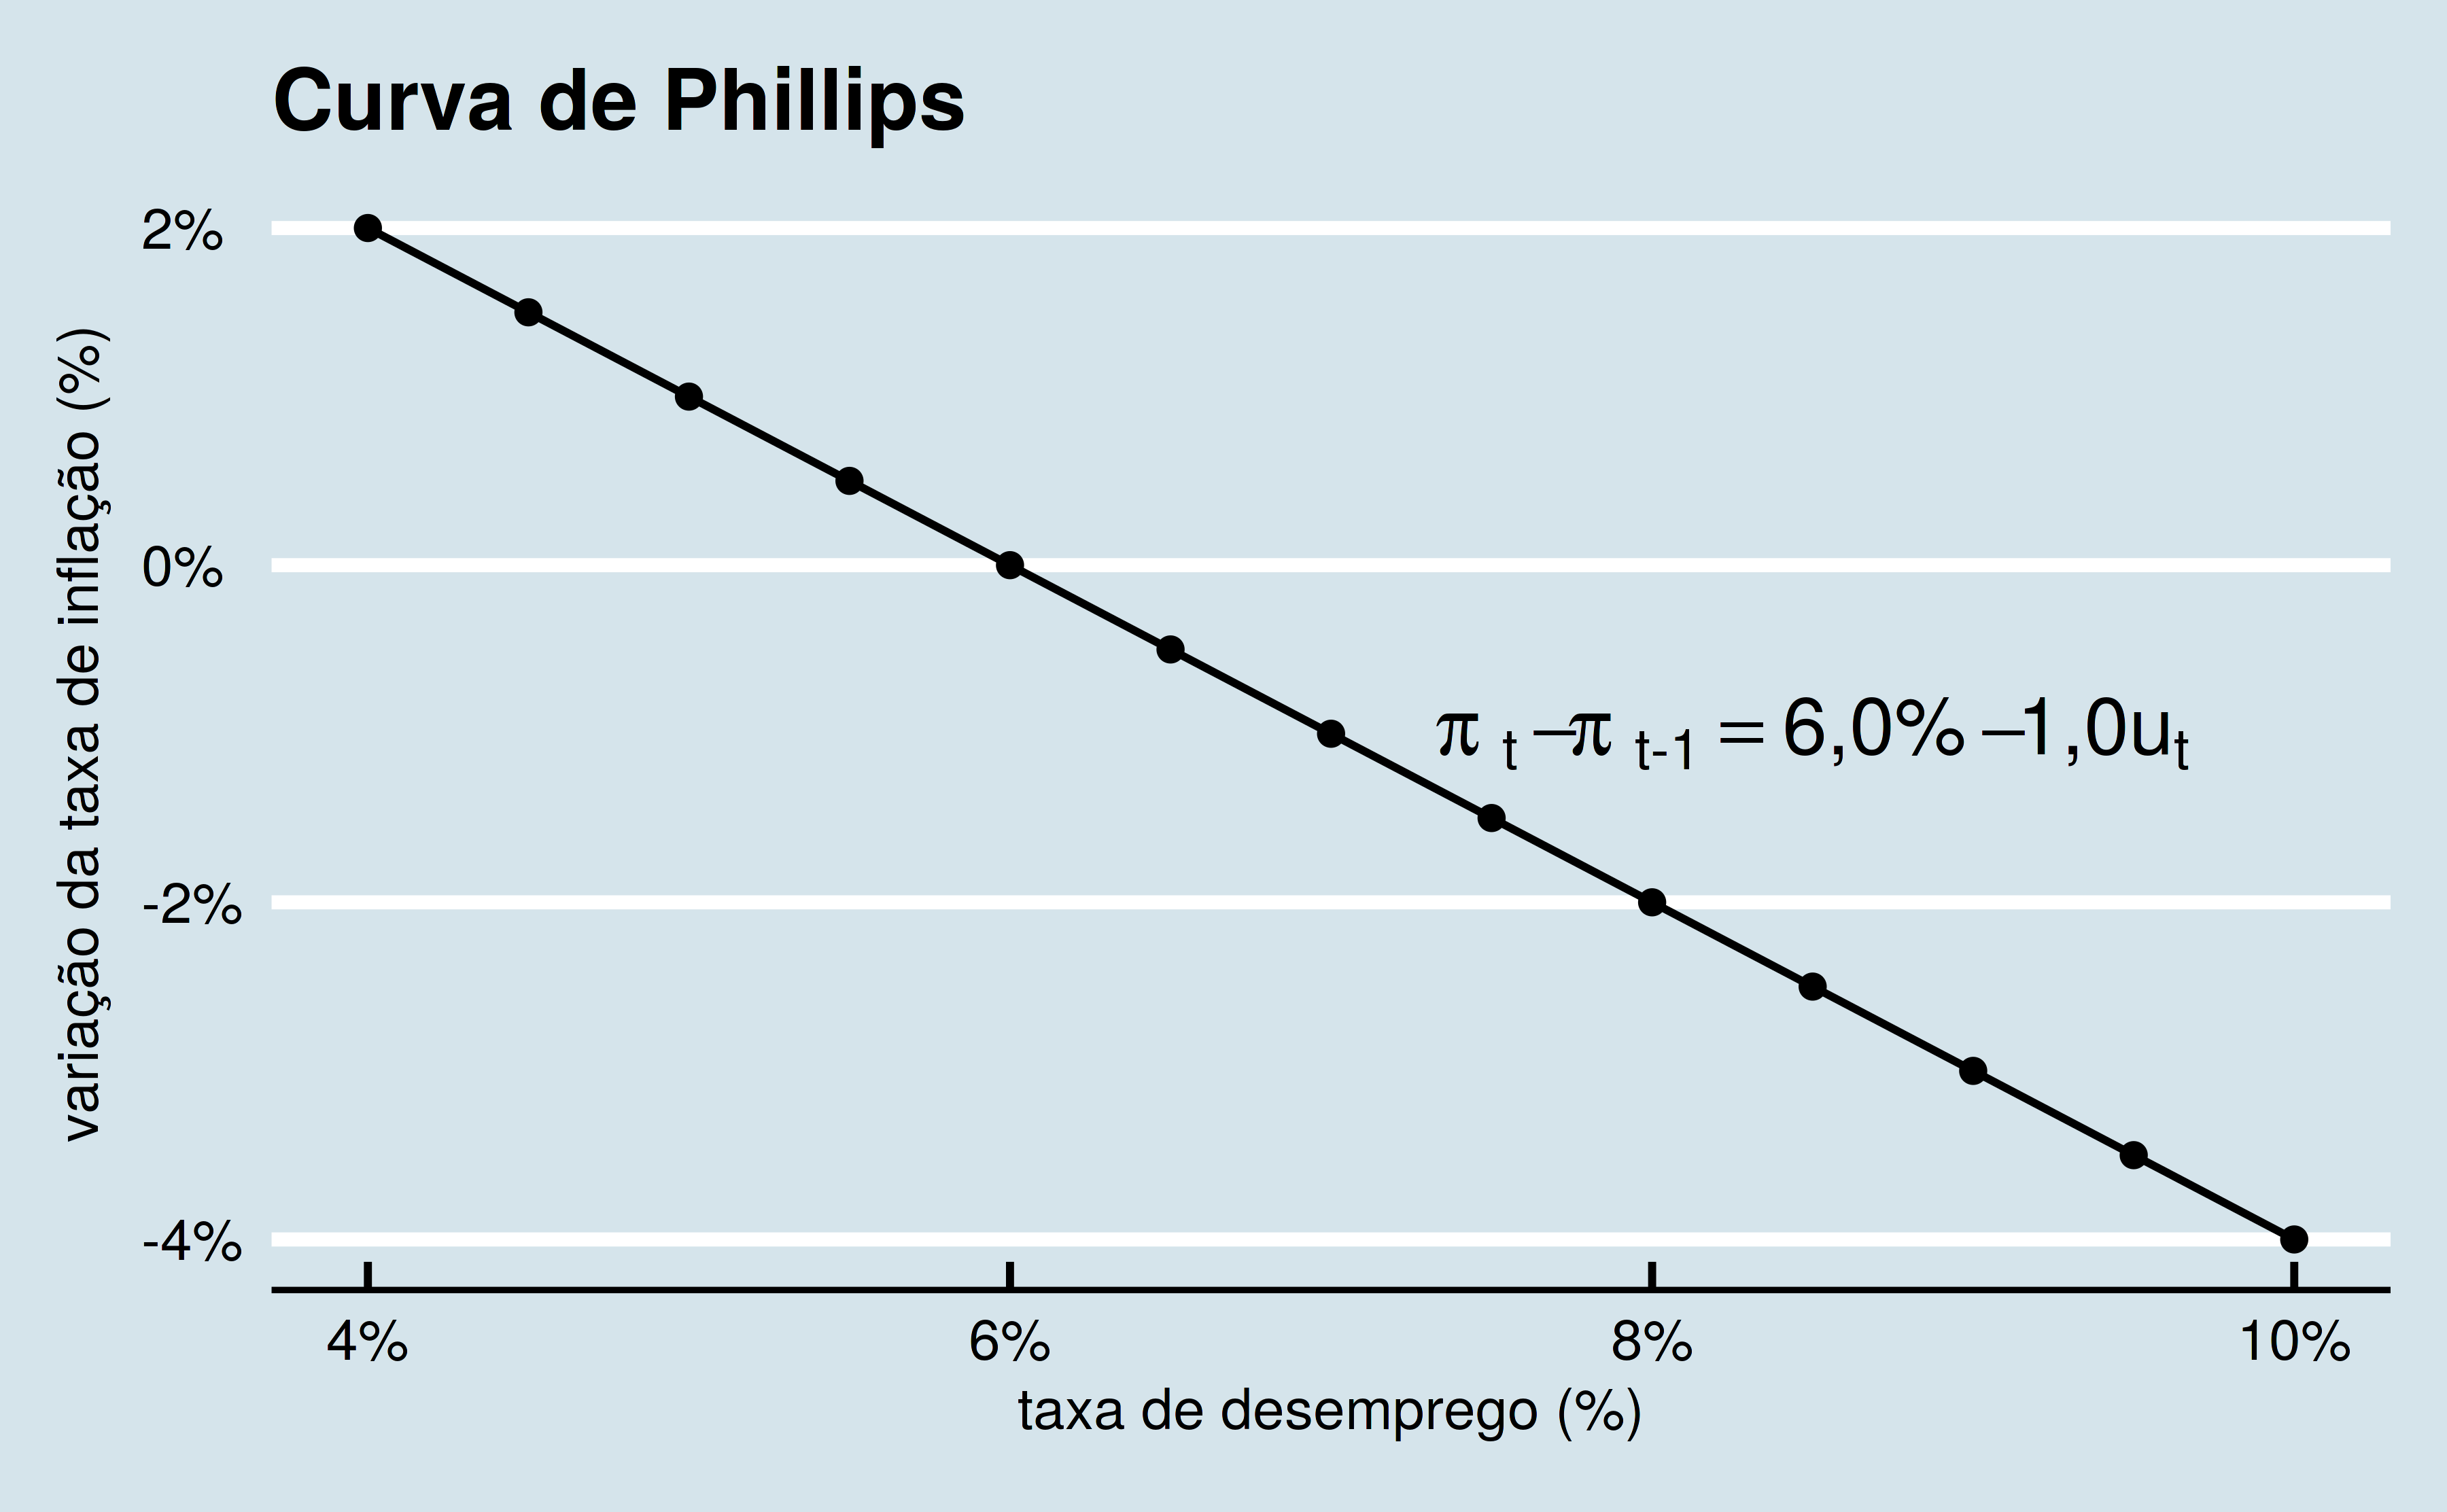
\includegraphics{imagens/phillips.png}
\caption{Curva de Phillips (exemplo)}\label{phillips}
\end{figure}

Fonte: \cite{blanchard}

Pode-se notar na \autoref{phillips} que a expressão de Phillips denota
um \emph{trade-off} entre inflação e desemprego, ou seja, quanto menor o
desemprego, mais a inflação sobe, e vice-versa.

Segundo \citeonline{wilher},

\subsubsection{Lei de Okun}\label{lei-de-okun}

Segundo \citeauthoronline{blanchard}, ``muitas decisões de política
macroeconômica envolvem dilemas entre perdas de curto prazo e ganhos no
longo prazo -- ou, simetricamente, entre ganhos de curto prazo e perdas
de longo prazo.''

De acordo com \citeauthoronline{blanchard}, ``os políticos ou os
formuladores de política econômica, (às vezes -- nota do autor), fazem o
que é melhor para si mesmos, e isso nem sempre é o melhor para o país.''

Pode ocorrer o caso, por exemplo, de que ``se o principal objetivo dos
políticos for agradar aos eleitores a fim de se reelegerem, qual será a
melhor política senão expandir a demanda agregada antes de uma eleição,
levando a um crescimento maior e a um desemprego menor''?

A \textbf{lei de Okun}, trata exatamente dos efeitos de um aumento no
produto sobre a taxa de desemprego. Elaborada por Arthur Okun
(economista e conselheiro do ex-predsidente norte-americano John
Kennedy) na década de 70, a lei de Okun relaciona a mudança no nível de
desemprego entre dois períodos (\(u_t - u_{t-1}\)) com a mudança na taxa
de crescimento do produto entre os mesmos dois períodos
(\(g_{yt} - \bar{g}_y\)), da seguinte forma \cite[p.~168]{blanchard}:

\[u_t - u_{t-1} = -\beta(g_{yt} - \bar{g}_y)\]

O coeficiente \(\beta\) varia de país para país e de época para época.

\begin{quote}
Pela lei de Okun, um crescimento do produto acima do crescimento normal
leva a um declínio da taxa de desemprego abaixo da taxa natural de
desemprego. Sabemos que, no médio prazo, a taxa de desemprego deve
aumentar e retornar à taxa natural de desemprego. Isso, por sua vez,
requer um crescimento do produto abaixo do normal por algum tempo
\cite[p.~492]{blanchard}.
\end{quote}

\subsubsection{Taxas de juros}\label{taxas-de-juros}

\paragraph{Taxa nominal de juros vs.~taxa real de
juros}\label{taxa-nominal-de-juros-vs.taxa-real-de-juros}

Segundo \citeauthoronline{blanchard}, taxa nominal de juros é aquela que
é ``expressa em termos de moeda nacional'' \cite[p.~274]{blanchard},
enquanto que a taxa real de juros é aquela que é ``expressa em termos de
uma cesta de bens'' \cite[p.~274]{blanchard}.

De acordo com \citeauthoronline{blanchard}, ``se representarmos a taxa
real de juros do ano \(t\) por \(r_t\), então, por definição, tomar
emprestado o equivalente a uma cesta de bens este ano corresponderá a
que você pague o equivalente a \(1 + r_t\) cestas de bens no próximo
ano.''

\paragraph{Relação entre taxa nominal e taxa real de
juros}\label{relacao-entre-taxa-nominal-e-taxa-real-de-juros}

Segundo \citeauthoronline{blanchard}, a taxa de juros real do ano \(t\),
\(r_t\) pode ser expressa em função da taxa de juros nominal do ano
\(t\), \(i_t\) e da inflação esperada \(\pi_{t+1}^e\) para o próximo
período, \(t+1\), através da fórmula abaixo \cite[p.~276]{blanchard}:

\[r_t\approx i_t - \pi_{t+1}^e\]

\paragraph{\texorpdfstring{Taxa de juros reais \emph{ex-ante} e taxa de
juros reais
\emph{ex-post}}{Taxa de juros reais ex-ante e taxa de juros reais ex-post}}\label{taxa-de-juros-reais-ex-ante-e-taxa-de-juros-reais-ex-post}

Segundo o Banco Central do Brasil, ``o comportamento da taxa real de
juros pode ser analisado sob duas óticas'':

A taxa real de juros \emph{ex-ante}, é aquela que ``compara a taxa de
juros contratada para determinado período com a taxa esperada de
inflação ao longo do mesmo período. Essa é a taxa mais relevante, pois é
a utilizada pelos agentes econômicos para a tomada de decisões.''
\cite[p.~52]{ri}

Já a taxa real de juros \emph{ex-post}, e aquele que ``compara a taxa de
juros acumulada durante um período no passado com a inflação efetiva
durante o mesmo período. Essa taxa reflete o que aconteceu no passado e
não as expectativas correntes'' \cite[p.~52-53]{ri}.

\paragraph{Taxa básica de juros ou taxa
Selic}\label{taxa-basica-de-juros-ou-taxa-selic}

A definição do Banco Central do Brasil para a nossa taxa básica de juros
(nominal), a taxa Selic, pode ser vista abaixo:

\begin{quote}
Define-se Taxa Selic como a taxa média ajustada dos financiamentos
diários apurados no Sistema Especial de Liquidação e de Custódia (Selic)
para títulos federais. Para fins de cálculo da taxa, são considerados os
financiamentos diários relativos às operações registradas e liquidadas
no próprio Selic e em sistemas operados por câmaras ou prestadores de
serviços de compensação e de liquidação (art. 1° da Circular n° 2.900,
de 24 de junho de 1999, com a alteração introduzida pelo art. 1° da
Circular n° 3.119, de 18 de abril de 2002)\footnote{\href{http://www.bcb.gov.br/htms/selic/conceito_taxaselic.asp}{www.bcb.gov.br/htms/selic/conceito\_taxaselic.asp}}
\end{quote}

\subsubsection{A função investimento e a eficiência marginal do
capital}\label{a-funcao-investimento-e-a-eficiencia-marginal-do-capital}

Para \citeonline[p.~3]{Bresser-Pereira1973}, ``a determinação da
variável estratégica a determinar o volume de investimentos torna-se de
extraordinária importância.''

Segundo \citeonline[p.~3]{Bresser-Pereira1973}, ``a tradição clássica de
dar primazia a taxa de lucros foi abandonada pelos neoclássicos, que
colocaram a taxa de juros no centro do seu sistema.'' Posteriormente,
foi Keynes quem ``restabeleceu, até um certo ponto, a importância da
taxa de lucros, através do conceito de eficiência marginal do capital.''

Para \citeauthoronline{Bresser-Pereira1973}, ``a teoria ortodoxa
\footnote{\citeonline{Bresser-Pereira1973} define como economistas ortodoxos os economistas neoclássicos e os keynesianos, no contexto do trabalho citado.}
sobre a função investimento afirma que a acumulação de capital depende
da taxa de lucro prevista (ou eficiência marginal do capital) da taxa de
juros, dado o nível da renda'', com uma relação inversa, ou seja, à
medida que aumenta o volume de investimentos, cai a eficiência marginal
do capital, conforme pode ser observado na \autoref{eficienciamarginal}
\cite[p.~4]{Bresser-Pereira1973}:

\begin{figure}
\centering
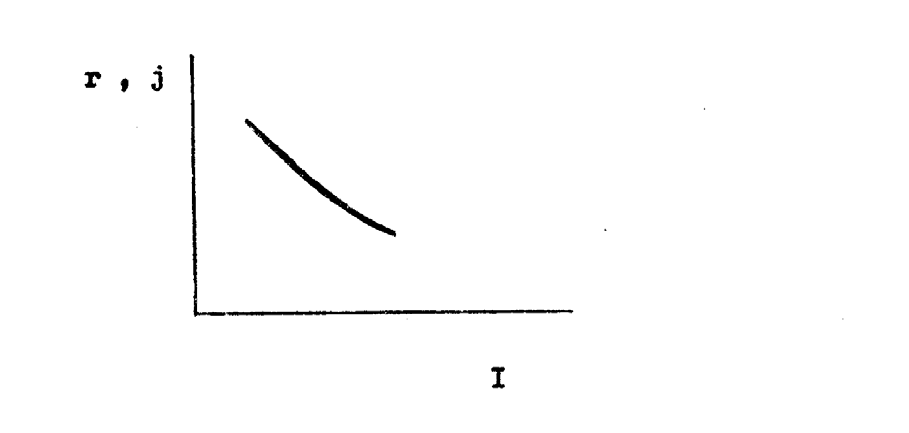
\includegraphics{imagens/Page-4-Image-1.png}
\caption{Eficiência Marginal do Capital e
Investimento}\label{eficienciamarginal}
\end{figure}

Fonte: \cite{Bresser-Pereira1973}

Uma das possíveis explicações para esta relação inversa pode ser vista
no trecho abaixo:

\begin{quote}
Há, portanto, uma relação inversa entre o volume dos investimentos e a
eficiência marginal do capital. Podemos, inclusive, imaginar que as
empresas ou os empresários disponham sempre de um ``estoque'' de
projetos de investimentos, com taxas diferentes e declinantes de lucro.
Quanto maiores fossem os investimentos efetivamente realizados, mais
seria preciso descer na escala de rentabilidade prevista dos projetos
{[}\ldots{}{]} Será interessante para a empresa investir enquanto ela
puder esperar do novo investimento um retorno superior ou pelo menos
igual ao da taxa de juros do mercado \cite[p.~5]{Bresser-Pereira1973}.
\end{quote}

A citação acima implica que também haverá uma relação entre a taxa de
juros de mercado e o volume de investimentos, novamente em uma relação
inversa, haja vista que quanto menor for a taxa de juros de mercado,
maior será o volume de investimentos.

A diferença básica entre a taxa de juros de mercado e a taxa de lucros
(ou eficiência marginal do capital), segundo
\citeauthoronline{Bresser-Pereira1973}, é que, enquanto a taxa de lucros
é dependente do volume de investimentos, a taxa de juros de mercado é
uma variável independente. ``Em outras palavras, é a variação dos
investimentos que leva à variação da eficiência marginal do capital,
enquanto que é a variação da taxa de juros que leva à variação do volume
de investimentos'' \cite[]{Bresser-Pereira1973}.

Segundo \citeauthoronline{Bresser-Pereira1973}, a eficiência marginal do
capital varia conforme o nível de otimismo dos empresários. A
``distinção entre a eficiência marginal do capital, dado um determinado
nível de otimismo dos empresários, \(r\), e a eficiência marginal do
capital com diferentes níveis de otimismo, quanto às suas perspectivas
de lucro, \(r’\)'', pode ser vista na \autoref{eficienciamarginal2}:
``fixada uma taxa de juros em um determinado nível \(j_1\), podemos,
então, deduzir graficamente uma nova função investimento, relacionando
positivamente o volume de investimentos, dado um nível de renda, com a
influência marginal do capital, \(r’\), a diferentes níveis de
otimismo'' \cite[p.~8]{Bresser-Pereira1973}:

\begin{figure}
\centering
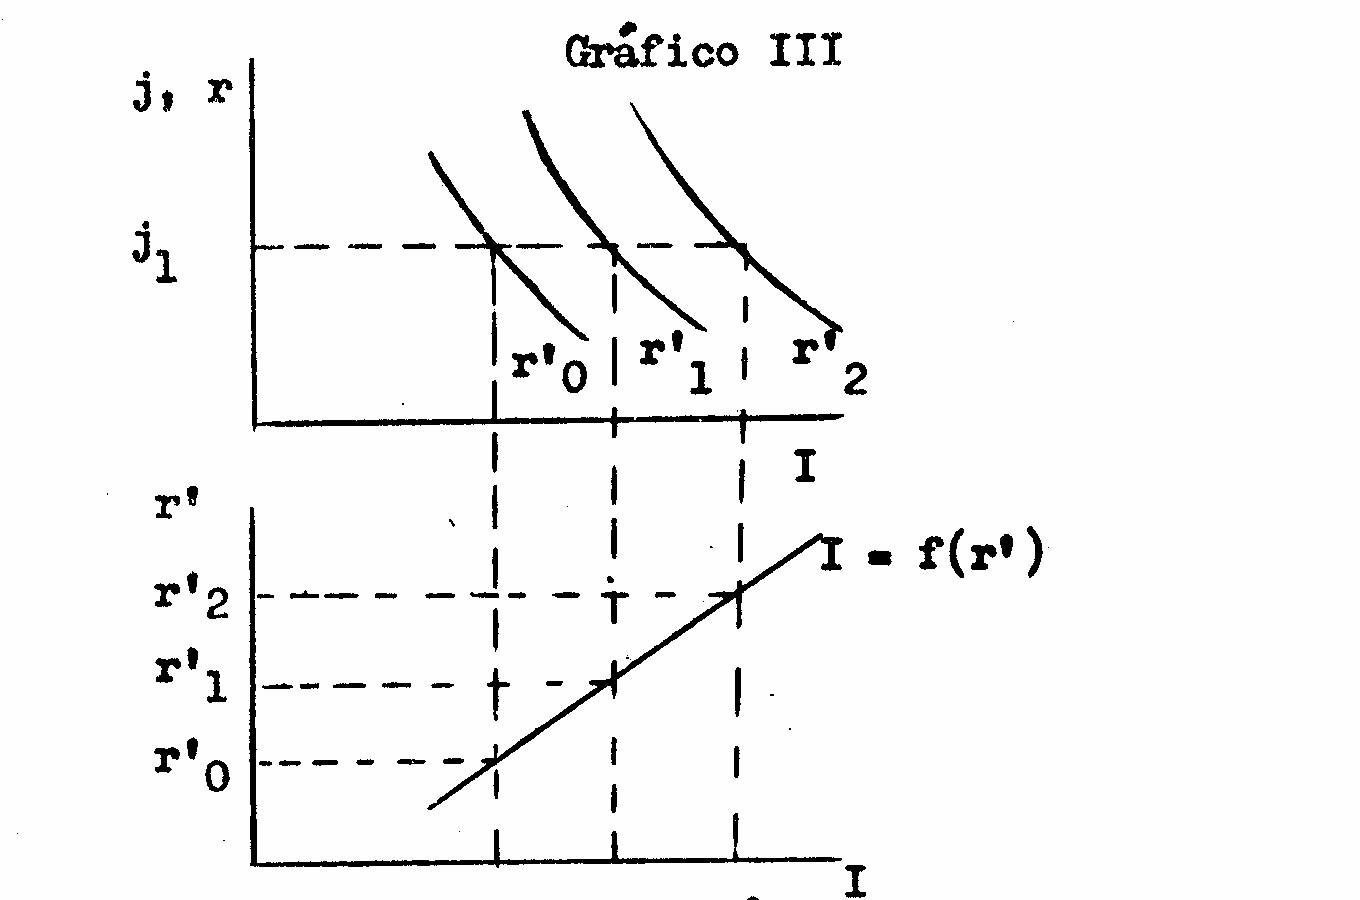
\includegraphics{imagens/imagem_final.png}
\caption{A nova função investimento}\label{eficienciamarginal2}
\end{figure}

Fonte: \cite{Bresser-Pereira1973}

\begin{quote}
Através dos mecanismos ortodoxos da política monetária e fiscal, e dos
mecanismos menos ortodoxos da política salarial, da política cambial, da
política fiscal ampliada, que inclui subsídios os mais variados, o
Governo tem condições crescentes de influenciar direta ou indiretamente
as perspectivas de lucro dos empresários. Por outro lado, as variações
no nível de segurança política para os investimentos, tão grandes no
mundo moderno, devem também fazer variar grandemente o nível de otimismo
dos empresários em relação a suas perspectivas de lucro
\cite[p.~9]{Bresser-Pereira1973}.
\end{quote}

Segundo \apudonline{rangel1956}{pereira}, ``a eficácia marginal do
capital das empresas com capacidade ociosa é negativa e, pela lógica, é
essa eficácia que deve orientar a taxa de juros.''

\subsubsection{Modelo IS-LM}\label{modelo-is-lm}

\paragraph{Relação IS}\label{relacao-is}

Segundo \citeauthoronline{blanchard}, a relação IS pode ser definida
como:

\begin{quote}
Relação IS é a condição de equilíbrio que afirma que a demanda por bens
deve ser igual à oferta de bens ou, de maneira equivalente, que o
investimento deve ser igual à poupança. Condição de equilíbrio do
mercado de bens \cite[p.~582]{blanchard}
\end{quote}

\paragraph{Curva IS}\label{curva-is}

De acordo com \citeauthoronline{blanchard}, a curva IS pode ser definida
como:

\begin{quote}
Curva IS é a curva negativamente inclinada que relaciona o produto à
taxa de juros. A curva corresponde à relação IS, a condição de
equilíbrio no mercado de bens \cite[p.~575]{blanchard}.
\end{quote}

\paragraph{Relação LM}\label{relacao-lm}

Para \citeauthoronline{blanchard}, ``relação LM é a condição de
equilíbrio que afirma que a demanda por moeda deve ser igual à oferta de
moeda. Condição de equilíbrio dos mercados financeiros''
\cite[p.~582]{blanchard}

\paragraph{Curva LM}\label{curva-lm}

De acordo com \citeauthoronline{blanchard}, a curva LM pode ser definida
como:

\begin{quote}
Curva LM é a curva positivamente inclinada que relaciona a taxa de juros
ao produto. A curva corresponde à relação LM, a condição de equilíbrio
para os mercados financeiros \cite[p.~575]{blanchard}.
\end{quote}

\subsubsection{Taxas de câmbio}\label{taxas-de-cambio}

\paragraph{Taxa de câmbio nominal}\label{taxa-de-cambio-nominal}

As taxas nominais de câmbio entre duas moedas podem ser expressas de
duas maneiras \cite[p.~354]{blanchard}:

\begin{itemize}
\tightlist
\item
  Como o preço da moeda nacional em termos de moeada estrangeira
\item
  Como o preço da moeda estrangeira em termos de moeda nacional
\end{itemize}

\paragraph{Taxa real de câmbio}\label{taxa-real-de-cambio}

Segundo \cite[p.~356]{blanchard}, a taxa real de câmbio expressa ``o
preço dos bens domésticos em termos de bens estrangeiros.''

Sendo \(E\) a taxa nominal de câmbio, \(P\) o nível de preços num país A
e \(P^*\) o nível de preços num país B, a taxa real de câmbio \(e\),
entre os países A e B pode ser expressa através da seguinte fórmula
\cite[p.~356]{blanchard}:

\[e = \frac{EP}{P^*}\]

\paragraph{Taxa de câmbio multilateral (taxa real de câmbio
multilateral)}\label{taxa-de-cambio-multilateral-taxa-real-de-cambio-multilateral}

É a ``taxa real de câmbio entre um país e seus parceiros comerciais,
calculada como a média ponderada das taxas reais de câmbio bilaterais.
Também chamada de taxa real de câmbio ponderada ou taxa real de câmbio
efetiva'' \cite[p.~583]{blanchard}.

\subsubsection{Dívida Pública Federal}\label{divida-publica-federal}

\paragraph{Dívida Bruta}\label{divida-bruta}

A dívida bruta é ``a soma dos itens que compõem o passivo financeiro do
governo federal'' \cite[p.~537]{blanchard}.

\paragraph{Dívida Líquida}\label{divida-liquida}

``Mais relevante, é a dívida líquida, ou, de modo equivalente, a
\emph{dívida em poder do público} \cite[p.~537]{blanchard}. Ou seja, em
outras palavras, a dívida pública mede a diferença entre o passivo total
e os ativos financeiros do governo\footnote{\href{http://epocanegocios.globo.com/Economia/noticia/2016/09/entenda-diferenca-entre-divida-publica-bruta-e-divida-liquida.html}{epocanegocios.globo.com/Economia/noticia/2016/09/entenda-diferenca-entre-divida-publica-bruta-e-divida-liquida.html}.}

\paragraph{Razão dívida-PIB}\label{razao-divida-pib}

\paragraph{Restrição orçamentária do
governo}\label{restricao-orcamentaria-do-governo}

Segundo \citeauthoronline{blanchard}, ``a restrição orçamentária do
governo relaciona a variação da dívida pública com o nível inicial da
dívida (que afeta o pagamento de juros), os gastos do governo atuais e
os impostos atuais'' \cite[p.525]{blanchard}

De acordo com \citeauthoronline{blanchard}, ``frequentemente, convém
decompor o déficit na soma de dois termos'':

\begin{itemize}
\tightlist
\item
  Pagamento de juros sobre a dívida, \(rB_{t-1}\).
\item
  A diferença entre os gastos e os impostos, \(G_t - T_t\), é chamado de
  \textbf{déficit primário} (ou, de maneira equivalente, \(T_t - G_t\) é
  chamado \textbf{superávit primário})
\end{itemize}

\subsection{Breve Histórico}\label{breve-historico}

Nesta seção pretendemos demonstrar a evolução das principais variáveis
macroeconômicas no Brasil, definidas na \autoref{sec:conceitos} desde a
implantação do Real, em julho de 1994.

\subsubsection{Principais variáveis macroeconômicas desde o Plano
Real}\label{principais-variaveis-macroeconomicas-desde-o-plano-real}

A variação do IPCA mensal, desde julho de 1994, pode ser vista na
\autoref{IPCA}.

\begin{figure}
\centering
\includegraphics[width=0.65000\textwidth]{imagens/IPCA_anual.png}
\caption{IPCA desde julho/1994}\label{IPCA}
\end{figure}

A \autoref{IPCA_anual} mostra os dados do IPCA anualizados, em forma de
barras.

\begin{figure}
\centering
\includegraphics[width=0.65000\textwidth]{imagens/IPCA_anual.png}
\caption{IPCA anual desde 1995}\label{IPCA_anual}
\end{figure}

A \autoref{cambio_nominal} mostra o gráfico da variação da cotação do
dólar em relação ao real, desde julho de 1994. Já a
\autoref{cambio_real} mostra a variação da taxa de câmbio real efetiva
no mesmo período.

\begin{figure}
\centering
\includegraphics[width=0.65000\textwidth]{imagens/cambio_nominal.png}
\caption{Taxa de câmbio nominal desde julho/1994}\label{cambio_nominal}
\end{figure}

\begin{figure}
\centering
\includegraphics[width=0.65000\textwidth]{imagens/cambio_real.png}
\caption{Taxa de câmbio real efetiva desde
junho/1994}\label{cambio_real}
\end{figure}

A \autoref{PIB} mostra a evolução do PIB real, em Reais do último ano,
enquanto a \autoref{PIB_anual} mostra a evolução da taxa de crescimento
anual do PIB real desde 1995.

\begin{figure}
\centering
\includegraphics[width=0.65000\textwidth]{imagens/PIB.png}
\caption{PIB em valores correntes - acumulado dos últimos 12
meses}\label{PIB}
\end{figure}

\begin{figure}
\centering
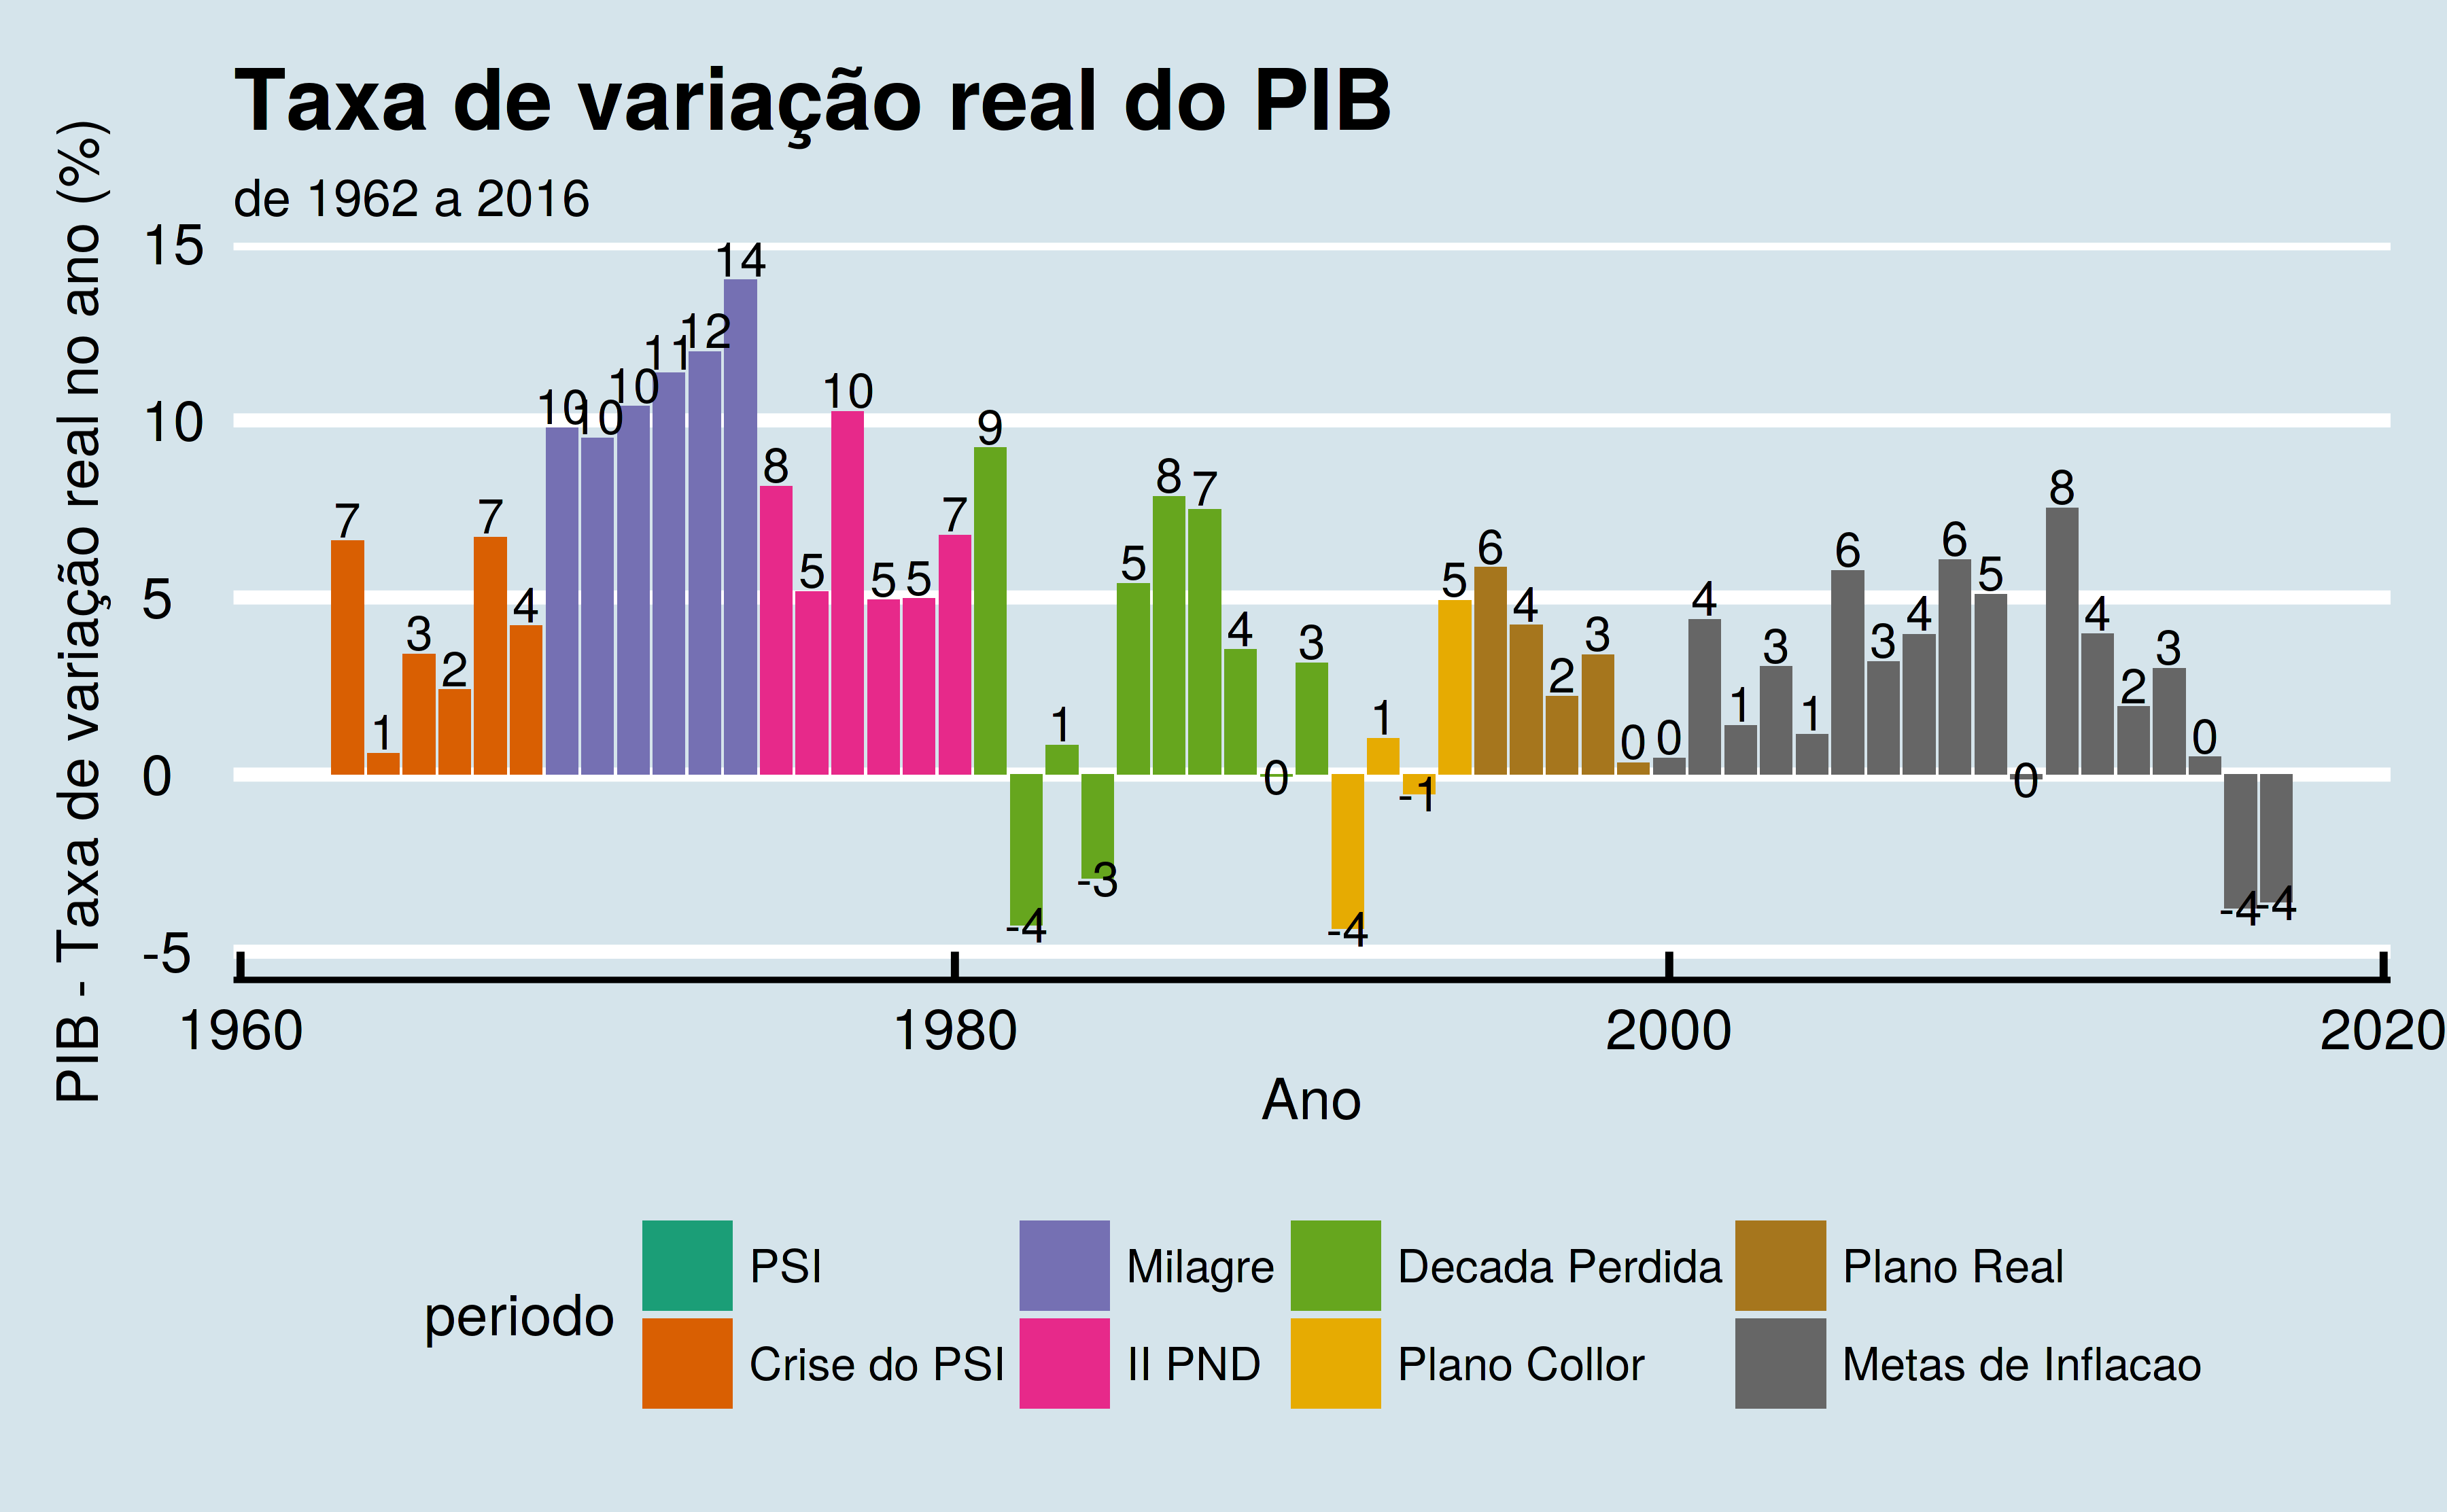
\includegraphics[width=0.65000\textwidth]{imagens/PIB_anual.png}
\caption{PIB anual desde 1995}\label{PIB_anual}
\end{figure}

A \autoref{selic} mostra a variação da taxa Selic desde julho/1994.

\begin{figure}
\centering
\includegraphics[width=0.65000\textwidth]{imagens/selic.png}
\caption{Taxa básica de juros desde julho/1994}\label{selic}
\end{figure}

A \autoref{juro_real} mostra a evolução da taxa de juros reais mensal
(\emph{ex-post}) do Brasil, desde julho de 1994.

\begin{figure}
\centering
\includegraphics[width=0.65000\textwidth]{imagens/juro_real.png}
\caption{Juros reais efetivos no Brasil desde julho/1994 (\% ao
mês)}\label{juro_real}
\end{figure}

A \autoref{juro_real_anual} mostra a evolução da taxa de juros reais
anualizada (\emph{ex-post}), desde junho de 1995, primeiro período onde
o efeito da hiperinflação prevalecente antes do plano real já havia se
dissipado.

\begin{figure}
\centering
\includegraphics[width=0.65000\textwidth]{imagens/juro_real_anual.png}
\caption{Juros reais efetivos no Brasil desde junho/1995 (\% ao
ano)}\label{juro_real_anual}
\end{figure}

A \autoref{divida_liquida} mostra a evolução da dívida líquida do setor
público desde a estabilização.

\begin{figure}
\centering
\includegraphics[width=0.65000\textwidth]{imagens/divida_liquida.png}
\caption{Dívida líquida do setor público desde julho/1994 (saldos em R\$
milhões)}\label{divida_liquida}
\end{figure}

Nas \Autoref{divida_liquida_GF,divida_liquida_BC} podem ser visualizadas
a dívida líquida do setor público em separado: a parte referente ao
Governo Federal e a parte referente ao BC.

\begin{figure}
\centering
\includegraphics[width=0.65000\textwidth]{imagens/divida_liquida_GF.png}
\caption{Dívida líquida do setor público desde julho/1994 - Gov.~Fed.
(saldos em R\$ milhões)}\label{divida_liquida_GF}
\end{figure}

\begin{figure}
\centering
\includegraphics[width=0.65000\textwidth]{imagens/divida_liquida_BC.png}
\caption{Dívida líquida do setor público desde julho/1994 - BC (saldos
em R\$ milhões)}\label{divida_liquida_BC}
\end{figure}

A \autoref{dividapib} mostra a evolução da razão da dívida líquida do
setor público (governo federal e banco central) em relação ao PIB.

\begin{figure}
\centering
\includegraphics[width=0.65000\textwidth]{imagens/dividapib.png}
\caption{Relação Dívida/PIB desde dez/2001}\label{dividapib}
\end{figure}

As \Autoref{desemprego1, desemprego2} mostram a evolução da taxa de
desemprego nas principais regiões metropolitanas, em duas séries
distintas, portanto incomparáveis, nos períodos de julho/1994 a dez/2002
e jan/2003 a fev/2016, respectivamente.

\begin{figure}
\centering
\includegraphics[width=0.65000\textwidth]{imagens/desemprego1.png}
\caption{Taxa de desemprego de julho/1994 a dez/2002}\label{desemprego1}
\end{figure}

\begin{figure}
\centering
\includegraphics[width=0.65000\textwidth]{imagens/desemprego2.png}
\caption{Taxa de desemprego de jan/2003 a fev/2016}\label{desemprego2}
\end{figure}

Por fim, a \autoref{dif_juros} mostra o diferencial de juros, ou seja, a
diferença entre a taxa de juros reais \emph{ex-ante} e a taxa de juros
neutra.

\begin{figure}
\centering
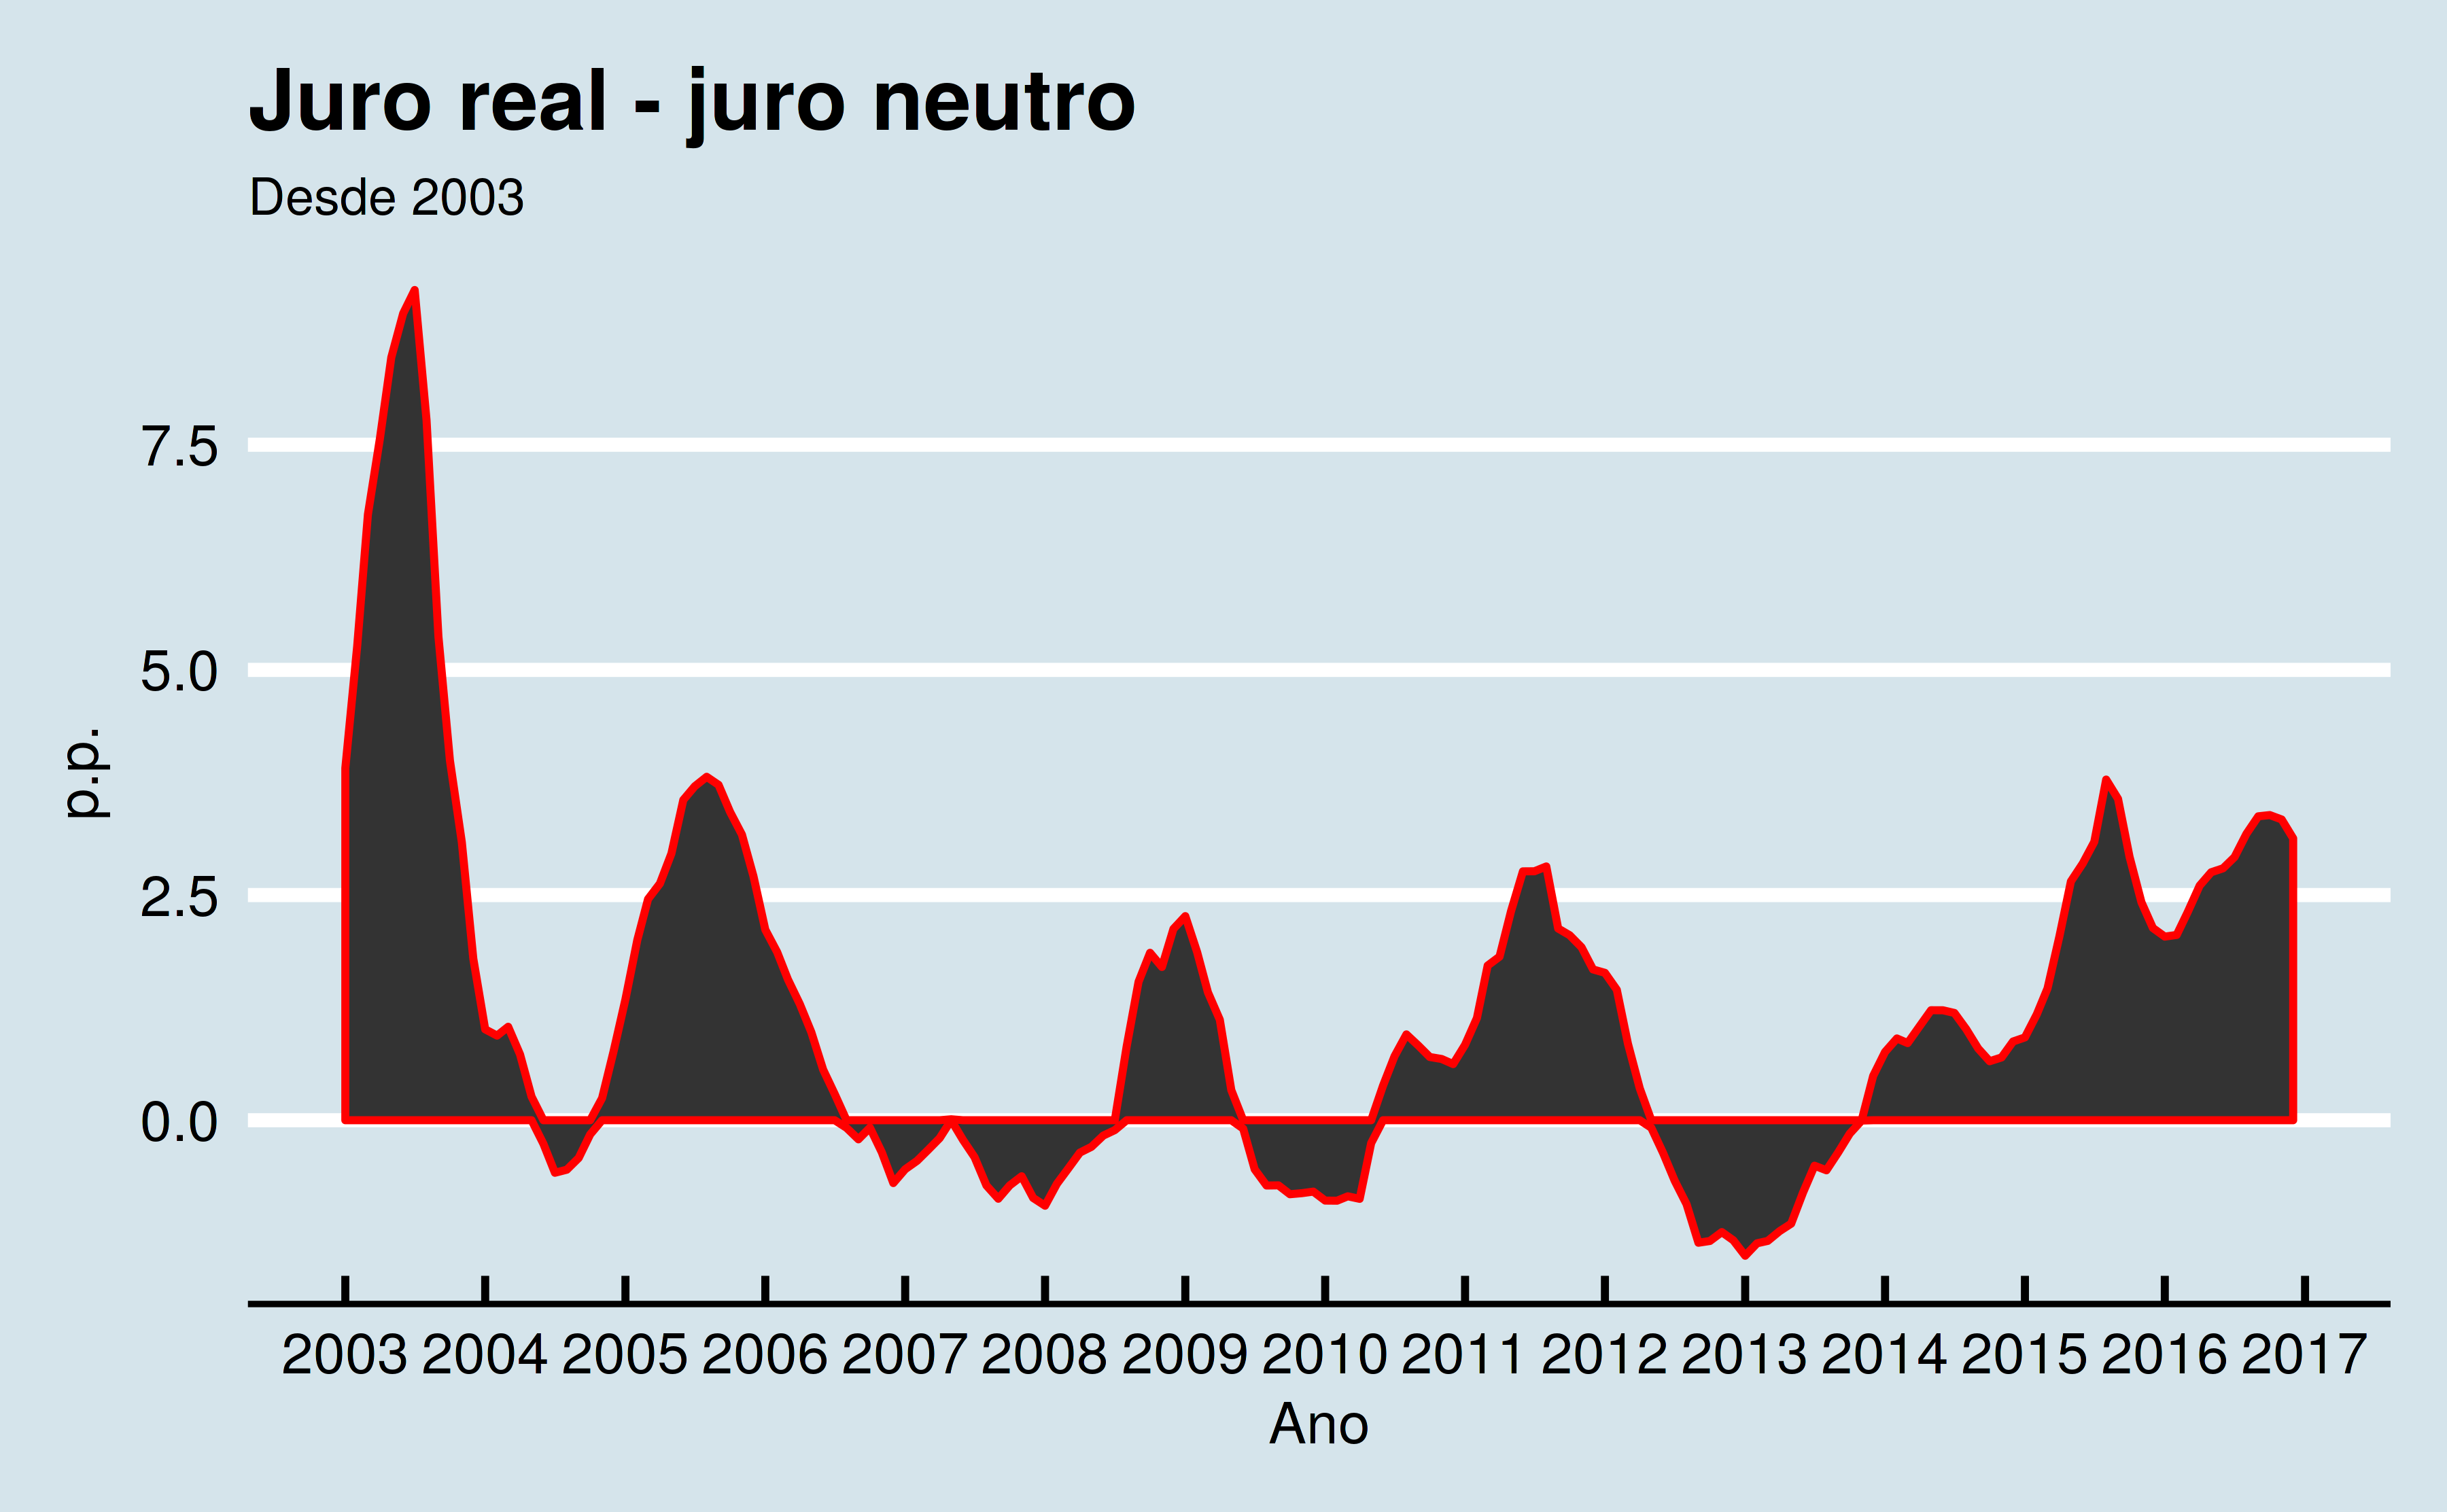
\includegraphics[width=0.65000\textwidth]{imagens/dif_juros.png}
\caption{Diferencial de juros (juros reais \emph{ex-ante} - juro
neutro)}\label{dif_juros}
\end{figure}

\section{Debate dos Juros no Brasil}\label{debate-dos-juros-no-brasil}

Recentemente teve início um intenso debate\footnote{\href{http://www.valor.com.br/debatedosjuros}{www.valor.com.br/debatedosjuros}}
sobre a eficácia do regime de metas de inflação no Brasil, sistema que é
a base da política monetária dos principais bancos centrais do mundo
desde meados dos anos 1990.

\subsection{André Lara Resende: primeiro
artigo}\label{andre-lara-resende-primeiro-artigo}

O debate teve início em janeiro de 2017 com artigo \textbf{Juros e
Conservadorismo Intelectual} \cite{resende1}\footnote{\href{http://www.valor.com.br/cultura/4834784/juros-e-conservadorismo-intelectual}{www.valor.com.br/cultura/4834784/juros-e-conservadorismo-intelectual}}

De acordo com \citeauthoronline{resende1}, ``desde a estabilização da
inflação crônica, com o Real -- e já se vão mais de 20 anos --, a taxa
básica de juros no Brasil causa perplexidade entre os analistas. Por que
tão alta?''

Ainda de acordo com \citeauthoronline{resende1}, embora diversas
explicações tenham sido elaboradas, ``nenhuma delas foi capaz de dar uma
resposta convincente e definitiva para a questão.''

A taxa básica de juros é o principal instrumento da política monetária.
``Juros mais altos reduzem a demanda agregada, desaquecem a economia e
moderam a inflação; juros mais baixos elevam a demanda agregada, aquecem
a economia e pressionam a inflação. Esta é a essência do mecanismo de
funcionamento da política monetária.'' Já ``quanto à inflação, sempre
houve controvérsia.''

\begin{quote}
O debate entre monetaristas e keynesianos, da segunda metade do século
XX, deu lugar a um consenso pós-keynesiano. Com o reconhecimento de que
instrumento usado pelos bancos centrais não são os agregados monetários,
mas sim a taxa de juros, e a adoção das metas para a inflação, chegou-se
ao atual relativo consenso sobre a condução da política monetária.
\end{quote}

De acordo com \citeauthoronline{resende1}, ``os modelos monetaristas,
cujo cerne era a TQM, expressa na equação MV = PY, provavelmente a
relação mais conhecida de toda a teoria econômica, pressupõem que a
velocidade de circulação da moeda, V, seja estável.''

No entanto, a partir da grande crise financeira de 2008, segundo
\citeauthoronline{resende1}, este consenso estaria definitivamente
ultrapassado: ``A experiência revolucionária dos bancos centrais do
mundo desenvolvido, desde a grande crise financeira de 2008, não deixa
mais dúvida: todos os modelos macroeconômicos que adotam alguma versão
da Teoria Quantitativa da Moeda (TQM) estão equivocados e devem ser
definitivamente aposentados'', haja vista que, depois de 2008 os
``bancos centrais aumentaram a oferta de moeda numa escala nunca
vista.''

``Logo, com o nível de atividade econômica, Y, mais ou menos constante,
um brutal aumento da quantidade de moeda, M, levaria a um aumento
proporcional do nível de preços, P, portanto, a uma explosão
inflacionária. Não foi o que ocorreu.''

Segundo \citeauthoronline{resende1}, os modelos neokeynesianos, ``até
hoje usados pelos bancos centrais'', tampouco explicam o comportamento
estável da inflação com taxas de juros tão baixas nos países
desenvolvidos:

\begin{quote}
Segundo a chamada Regra de Taylor, para estabilizar a inflação, o juro
deve ser reduzido ou aumentado mais do que proporcionalmente e de
maneira inversa ao movimento observado na inflação. Se a política
monetária for passiva, ou seja, não reagir de maneira inversa e mais do
que proporcional aos movimentos observados na taxa de inflação, a
inflação ficará instável. Assim que a taxa de juros atingisse, como de
fato atingiu, um limite inferior nominal, próximo de zero, o processo
deflacionário se tornaria incontrolável. Também não foi o que ocorreu.
\end{quote}

\citeauthoronline{resende1} finalmente afirma que ``o único modelo
compatível com a estabilidade observada da inflação é o neokeynesiano
mais recente, na sua vertente neo-fisheriana, utilizado apenas na
fronteira acadêmica, pois além de sérias complicações analíticas,
inverte a relação entre juros e inflação. A condução da política
monetária estaria assim, há décadas, seriamente equivocada.''

\subsection{Marcos Lisboa e Samule Pessoa: a
réplica}\label{marcos-lisboa-e-samule-pessoa-a-replica}

\citeauthoronline{lisboapessoa} foram os primeiros a rebater Resende, em
20/01/2017, também no Jornal Valor Econômico, com o artigo \textbf{Nada
de novo no debate monetário no Brasil} \cite{lisboapessoa} \footnote{\href{http://www.valor.com.br/cultura/4842254/nada-de-novo-no-debate-monetario-no-brasil}{www.valor.com.br/cultura/4842254/nada-de-novo-no-debate-monetario-no-brasil}}.

Segundo \citeauthoronline{lisboapessoa}, apesar da proposição de
Cochrane, ``que aumentos da taxa nominal de juros podem ajudar à
recuperação da economia americana'', ou seja, o contrário do que
preconiza a teoria monetária padrão, ``seria desejável uma robusta
evidência empírica para extrair dessa possibilidade uma proposta de
condução alternativa de política monetária no Brasil'', haja vista que
``do formulador da política pública, espera-se a análise da melhor
evidência disponível para adotar medidas que podem afetar a muitos. A
política monetária requer o cuidado do enfermeiro'', e citam evidências
históricas da eficácia da política monetária tradicional no combate a
inflação:

\begin{quote}
Em agosto de 1979, Paul Volcker assumiu a presidência do banco central
americano (Fed). A inflação estava em cerca de 9\% ao ano, e se esperava
que pudesse aumentar ainda mais. Volcker iniciou um longo período de
combate à inflação e a taxa básica de juros chegou a ultrapassar 18\% ao
ano. A política monetária vinha de pouco mais de uma década de leniência
com a inflação, acomodando choques de oferta, como o do petróleo. Essa
longa leniência contaminou as expectativas e tornou o combate à inflação
muito mais custoso. Havia dúvidas sobre o comprometimento do Fed com a
estabilização da economia e foram necessários quase quatro anos para que
a inflação cedesse.
\end{quote}

\citeauthoronline{lisboapessoa} argumentam que até ``pode-se criticar a
qualidade da execução da estratégia do modelo padrão em vários momentos.
Mas não parece haver evidência de que cortes abruptos de juros reduzam a
inflação por aqui.''

Pelo contrário, segundo os mesmos a ``condução da política monetária em
2011 ilustra as consequências da intervenção motivada por um diagnóstico
equivocado'', se referindo ao período no qual o Bacen reduziu a taxa de
juros básica aos níveis historicamente mais baixos desde a
estabilização.

\citeauthoronline{lisboapessoa} veem a condução heterodoxa da política
monetárias dos países desenvolvidos a partir de 2008 motivada pela
impossibilidade de utilização do modelo padrão da política monetária
``quando a taxa neutra de juros se aproxima de zero'', explicitam os
mecanismos que fariam, segundo a teoria de Cochrane, o aumento dos juros
ocasionar o aumento da inflação, e concluem que ``nada indica que a
conjectura seja válida para a economia brasileira.'' Pelo contrário,
argumentam que ``os testes empíricos disponíveis indicam que o modelo
padrão funciona por aqui: aumento da taxa real de juros reduz a demanda,
como ilustra a atual queda da inflação em contraposição ao afrouxamento
da política monetária a partir de agosto de 2011.''

\subsection{André Lara Resende: a
tréplica}\label{andre-lara-resende-a-treplica}

\citeauthoronline{resende2}, em 27/01/2017, volta ao debate com o artigo
\textbf{Teoria, prática e bom senso} \cite{resende2}\footnote{\href{http://www.valor.com.br/cultura/4849060/teoria-pratica-e-bom-senso}{www.valor.com.br/cultura/4849060/teoria-pratica-e-bom-senso}}
e afirma que ``no Brasil, a inflação é muito pouco sensível à taxa de
juros. As razões da ineficácia da política monetária são muitas e
controvertidas, mas a baixa sensibilidade da inflação à taxa de juros é
indiscutível, uma unanimidade'' e que ``o custo fiscal da política
monetária não é irrelevante.''

Segundo \citeauthoronline{resende2}, ainda, ``da política monetária só
se pode pedir que evite maiores flutuações do nível de atividade e
balize as expectativas de inflação. Sem credibilidade fiscal a política
monetária é impotente.''

\subsection{José Júlio Senna: xxxxxxx}\label{jose-julio-senna-xxxxxxx}

\citeauthoronline{senna}\footnote{\href{http://www.valor.com.br/cultura/4864408/taxa-de-juros-e-inflacao}{www.valor.com.br/cultura/4864408/taxa-de-juros-e-inflacao}},
em artigo de 10/02/2017, \textbf{Taxa de Juros e Inflação} \cite{senna},
refuta a linha de argumentação de Cochrane, haja vista que ``as
abordagens teóricas criticadas há décadas funcionam bem para explicar
fenômenos monetários, como também é possível reconciliá-las com os
resultados observados após a crise financeira.''

Segundo \citeauthoronline{senna}, ``é fácil constatar que fenômenos
extraordinários ocorridos nesse período prejudicaram o funcionamento dos
instrumentos monetários clássicos, o que não os desqualifica para outras
situações'', e cita a análise de Richard Koo sobre o Japão, segundo o
qual ``muitas empresas passaram a privilegiar a redução da dívida,
seguraram investimentos e fugiram de novos empréstimos, mesmo diante de
juro zerom, o que causou a contração do multiplicador bancário.'' Por
conta desta contração do multiplicador bancário, o programa, ``primeiro
QE de que se tem notícia, não funcionou como o esperado.''

Para \citeauthoronline{senna}:

\begin{quote}
a crise financeira recente aparentemente provocou fenômeno semelhante em
grande parte do mundo desenvolvido. Desta vez, não apenas empresas, mas
também famílias perceberam-se excessivamente endividadas, passando a
priorizar o ajustamento patrimonial, sendo assim, também não há como a
inflação `explodir' em consequência de QE.
\end{quote}

Ainda, \citeauthoronline{senna} explica o motivo de não ter havido
deflação, que segundo o modelo neokeynesiano e de acordo com Cochrane,
ocorreria com a ocorrência de juro zero: ``cabe notar que o QE e outras
formas de estímulo não produziram o efeito previsto, mas é razoável
supor que tiveram algum impacto, sustentando a demanda. Seria esta a
razão de não ter havido deflação.''

\citeauthoronline{senna} também considera ``a aplicação da teoria (de
Cochrane) à realidade brasileira parece ainda mais inapropriada'', haja
vista que ``Cochrane não faz referência a juros reais, aspecto que
verdadeiramente se debate no Brasil. Sua análise diz respeito a juros
nominais\}, e rebate Resende dizendo que''não é válido basear a defesa
de juros baixos na experiência do QE do mundo desenvolvido. Primeiro
porque fatores extraordinários interferiram no resultado dessa
experiência. Segundo porque se trata de situação que nada tem a ver com
a realidade brasileira" e também discordando da afirmação de
\citeauthoronline{resende2} de que a inflação no Brasil seria muito
pouco sensível a variações de taxa de juros: ``os números, porém, não
sustentam essa afirmação. Nos últimos anos, tivemos vários ciclos de
alta e de baixa da taxa Selic. Em todos esses episódios a inflação
reagiu de acordo com o raciocínio tradicional, caindo em resposta às
fases de alta e subindo em resposta aos ciclos de baixa, com defasagem
variável.''

\subsection{Francisco Lopes: xxxxxxx}\label{francisco-lopes-xxxxxxx}

Em artigo de 17/02/2017, \textbf{André Cochrane e a teoria fiscal dos
preços}\footnote{\href{http://www.valor.com.br/cultura/4872458/andre-cochrane-e-teoria-fiscal-dos-precos}{www.valor.com.br/cultura/4872458/andre-cochrane-e-teoria-fiscal-dos-precos}},
\citeonline{lopes} afirma que ``a teoria keynesiana moderna, que é
utilizada por todos os bancos centrais, não encontra maior dificuldade
para explicar os fatos'', e que:

\begin{quote}
Cochrane utiliza uma versão simplificada da teoria para demonstrar que,
quando a taxa de juros de curto prazo é reduzida até zero, só existem
duas possibilidades: ou a taxa de inflação volta a subir em direção à
meta ou ocorre um processo ilimitado de deflação. Como nada disso teria
ocorrido na experiência americana depois que a taxa de juros foi
reduzida a praticamente zero ao fim de 2008, a conclusão é de que
precisamos uma reformulação fundamental da teoria, e Cochrane sugere a
alternativa da teoria fiscal dos preços.
\end{quote}

Para \citeauthoronline{lopes} , ``os números de inflação para os EUA
estão longe de justificar o radicalismo de Cochrane e em 2016 a taxa de
inflação já convergiu, sim, para a meta do Fed de 2\% ano.'' Não seria
correto, portanto, ``dizer que a política monetária americana com taxa
de juros próxima de zero não atingiu seu objetivo de colocar a inflação
na meta.'' Esta convergência da inflação para a meta teria se dado de
maneira lenta posto que ``nesses anos havia uma taxa de desemprego na
faixa de 7 a 9\%, o mercado imobiliário continuava em crise e as
famílias provavelmente ainda estavam reduzindo suas despesas pessoais
para ajustar seus endividamentos. Logo existiam forças importantes
operando no sentido de impedir a elevação da taxa de inflação.''

\citeauthoronline{lopes} também argumenta que ``em 2014 e 2015, quando a
inflação caiu abaixo de 1\%. Essa desaceleração ocorreu junto a gradual
eliminação do relaxamento quantitativo (QE), portanto em princípio com
um aperto na política monetária, mas esta não nos parece ser a melhor
explicação.'' Para Lopes, ``o fator determinante foi uma brusca queda
nos preços internacionais de commodities, com a cotação do petróleo
Brent, por exemplo, caindo cerca de 70\% entre meados de 2014 e fim de
2015.'' Já quando a situação se inverteu ``em 2016 alguns preços
internacionais de commodities voltaram a subir (como 40\% para o
petróleo e 20\% para os metais), o que certamente contribuiu para a
elevação da taxa de inflação.'' E então conclui: ``desde 2009 a política
monetária americana foi efetivamente expansionista, ainda que diversos
fatores tenham contribuído para um retorno relativamente gradual em
direção à meta.''

Quanto a possibilidade de deflação ilimitada defendida por Cochrane
quando a política monetária atinge a restrição de piso zero (ou seja,
quando a taxa de juros básica da economia atinge o zero),
\citeauthoronline{lopes} explica que ``pode acontecer que um banco
central operando uma meta de inflação seja levado a reduzir a taxa
nominal de juros até zero sem que consiga levar o nível de atividade a
uma posição suficiente para reverter uma tendência generalizada à
deflação dos preços. Devido ao piso zero, a economia não consegue sair
da posição deflacionária apenas através da política monetária e vai
depender para isso de um estímulo fiscal.''

Segundo \citeauthoronline{lopes} , a teoria fiscal dos preços (TFP)
parece estar incompleta e afirma que não está claro qual é o mecanismo
de mercado que produz o movimento do índice de preços derivado das
mudanças na parte fiscal, argumentando que ``parece mais razoável supor
que o impacto será no mercado secundário de títulos da dívida pública, o
que sugere que está faltando algo na equação básica da teoria.''

Para ele ``a conclusão é de que a teoria fiscal de preços não é uma nova
teoria para a inflação, mas apenas uma teoria fiscal da taxa longa de
juros.''

\subsection{Nelson Barbosa: xxxxxxx}\label{nelson-barbosa-xxxxxxx}

Em 24/02/2017, \citeauthoronline{barbosa} inicia seu artigo,
\textbf{Taxa real de juro: evolução e perspectivas}\footnote{\href{http://www.valor.com.br/cultura/4879800/taxa-real-de-juro-evolucao-e-perspectivas}{www.valor.com.br/cultura/4879800/taxa-real-de-juro-evolucao-e-perspectivas}}
\cite{barbosa}, com a afirmação que ``o Brasil tem a mais alta taxa
básica de juro do mundo em termos reais'', expõe os \ldots{}

Posteriormente, muitos outros economistas proeminentes de vários
espectros políticos entraram no debate, como \citeauthoronline{loyo},
\citeauthoronline{nakano}, \citeauthoronline{belluzo},
\citeauthoronline{coutinho} e outros.


\end{document}
